\documentclass{ceurart}

\usepackage{acronym}
\usepackage{subcaption}
\usepackage{dirtree}
\usepackage{listings}
\usepackage{float}
\usepackage{lmodern}
\restylefloat{table}



\lstset{frame=tb,
  language=Java,
  aboveskip=3mm,
  belowskip=3mm,
  showstringspaces=false,
  columns=flexible,
  basicstyle={\small\ttfamily},
  numbers=none,
  breaklines=true,
  breakatwhitespace=true,
  tabsize=3
}

\renewcommand{\acffont}[1]{\textsl{#1}}


%%
%% end of the preamble, start of the body of the document source.
\begin{document}

%%
%% Rights management information.
%% CC-BY is default license.
\copyrightyear{2023}
\copyrightclause{Copyright for this paper by its authors.\\
  Use permitted under Creative Commons License Attribution 4.0
  International (CC BY 4.0).}

%%
%% This command is for the conference information
\conference{``Search Engines'', course at the master degree in ``Computer Engineering'', Department of Information Engineering, and at the master degree in ``Data Science'', Department of Mathematics ``Tullio Levi-Civita'', University of Padua, Italy. Academic Year 2022/2023}

%%
%% The "title" command
\title{SEUPD@CLEF: Team CLOSE}

%%
%% The "author" command and its associated commands are used to define
%% the authors and their affiliations.
\author[1]{Antolini Gianluca}[%
email=gianluca.antolini@studenti.unipd.it
]

\author[1]{Boscolo Cegion Nicola}[%
email=nicola.boscolocegion.1@studenti.unipd.it
]

\author[1]{Cazzaro Mirco}[%
email=mirco.cazzaro@studenti.unipd.it
]

\author[1]{Martinelli Marco}[%
email=marco.martinelli.4@studenti.unipd.it
]

\author[1]{Safavi Seyedreza}[%
email=seyedreza.safavi@studenti.unipd.it
]

\author[1]{Shami Farzad}[%
email=farzad.shami@studenti.unipd.it
]

\address[1]{University of Padua, Italy}


%%
%% The abstract is a short summary of the work to be presented in the
%% article.
\begin{abstract}
  This paper presents the work of the \textit{CLOSE} group, a team of students from the University of Padua, Italy, for the 2023 \ac{CLEF} Task 1 \cite{cleflongeval}.
  Our work involved developing an Information Retrieval system that can handle changes in data over time while maintaining high performance.
  We first introduce the problem as stated by \ac{CLEF} and then describe our system, explaining the different methodologies we implemented.
  We provide the results of our experiments and analyze them based on the choices we made regarding various techniques.
  Finally, we propose potential avenues for future improvement of our system.
\end{abstract}

%%
%% Keywords. The author(s) should pick words that accurately describe
%% the work being presented. Separate the keywords with commas.
\begin{keywords}
  Information Retrieval \sep
  Search Engines \sep
  Longitudinal Evaluation \sep
  Model Performance
\end{keywords}

%%
%% This command processes the author and affiliation and title
%% information and builds the first part of the formatted document.
\maketitle


\enlargethispage{2\baselineskip}
\section{Introduction}
\label{sec:introduction}

Recent research has shown that the performance of information retrieval systems can deteriorate over time as the data they are trained on becomes less relevant to current search queries. 
This problem is particularly acute when dealing with temporal information, as web documents and user search preferences evolve over time. 
In this paper, we propose a solution to this problem by developing an information retrieval system that can adapt to changes in the data over time, while maintaining high performance.

Our approach involves using the training data provided by \textit{Qwant}~\cite{qwant} search engine, which includes user searches and web documents in both French and English.
We believe that this data will enable our system to better adapt to changes in user search behavior and the content of web documents.

The remainder of this paper is organized as follows: 
Section~\ref{sec:methodology} describes our approach in more detail, including the different techniques we used. 
Section~\ref{sec:setup} explains our experimental setup, including the datasets and evaluation metrics we used. 
Section~\ref{sec:results} presents our main findings and analyzes them based on the choices we made regarding various techniques. 
Finally, Section~\ref{sec:conclusion} summarizes our conclusions and outlines potential avenues for future work.

\section{Methodology}
\label{sec:methodology}

\subsection{General Overview of Our IR System}
In the development of our \ac{IR} system, we followed the traditional \textit{Y model}, represented in the figure below.

\begin{figure}[!h]
    \centering
    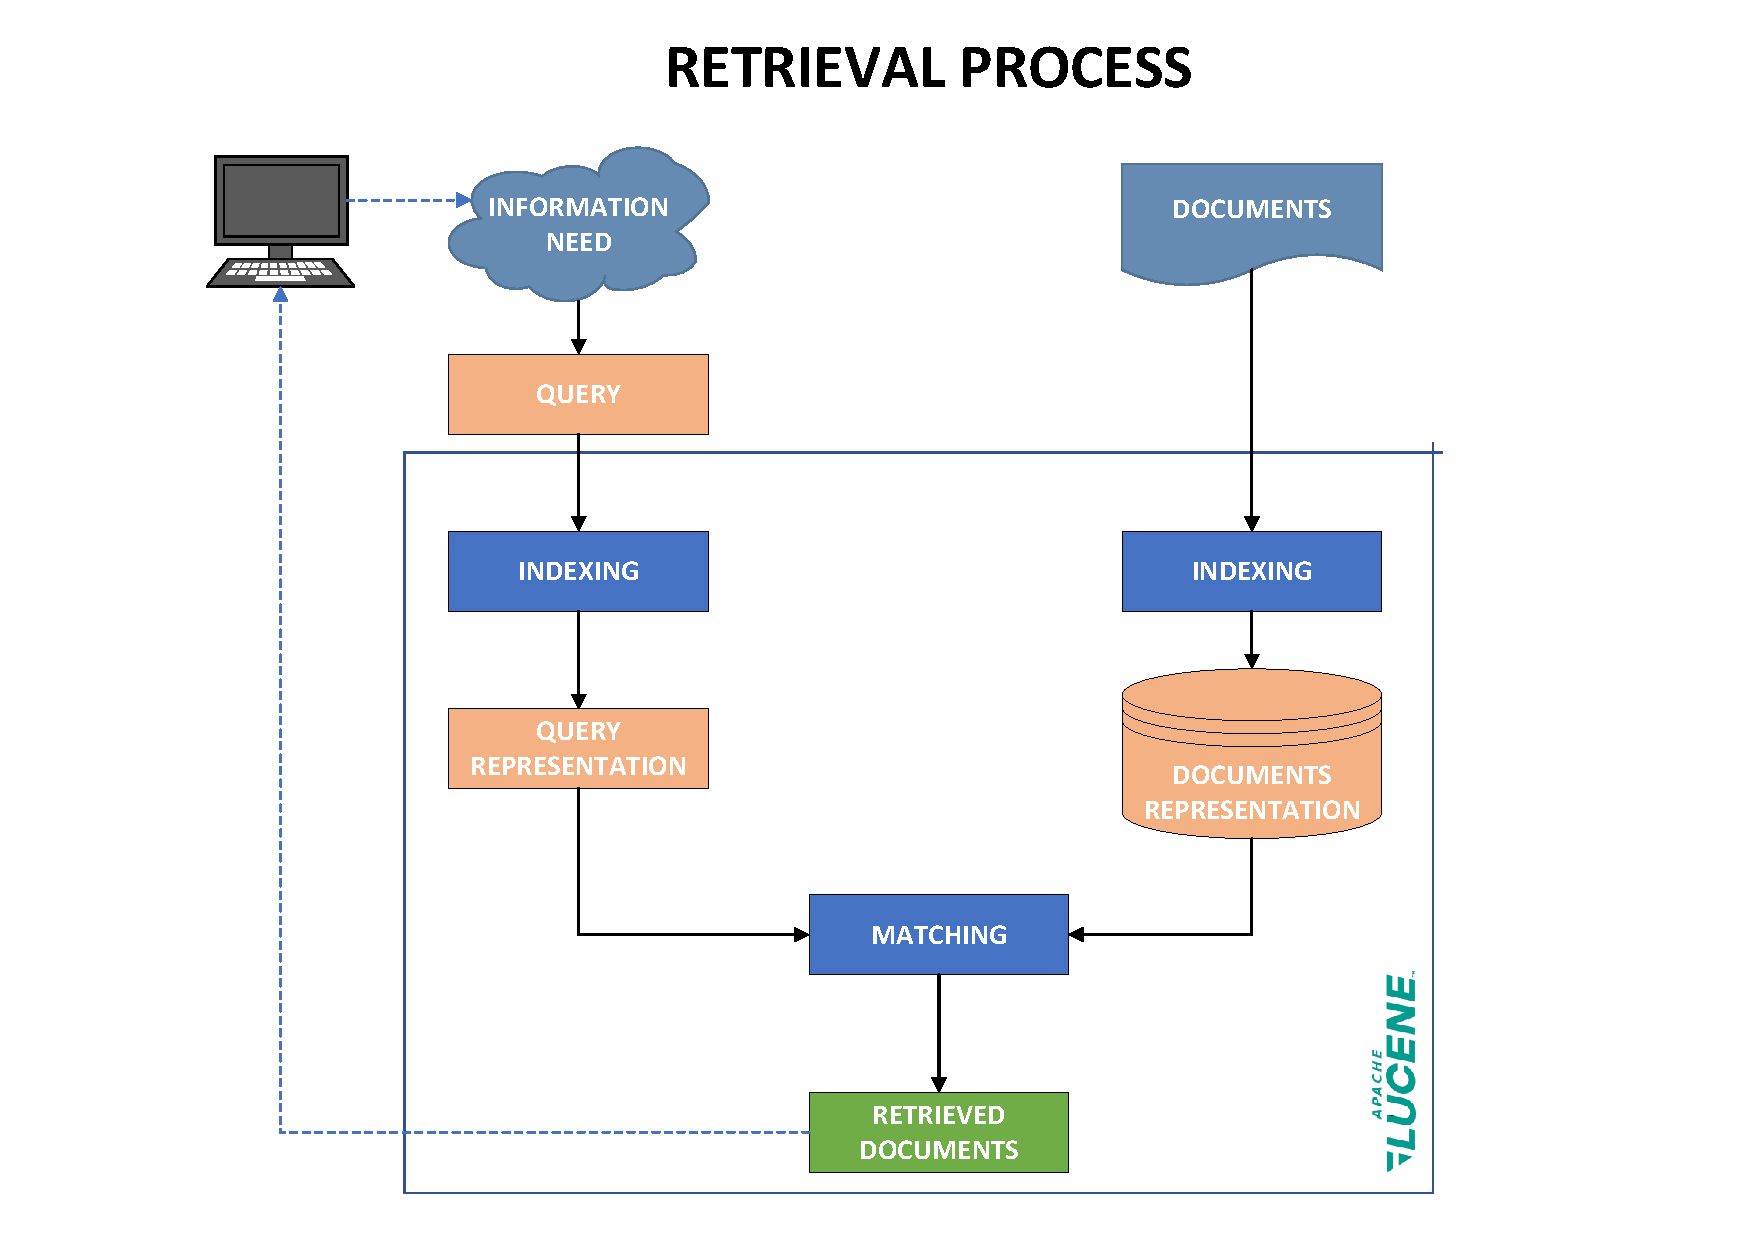
\includegraphics[width=0.9\linewidth]{figure/Y.pdf} 
    \caption{Apache Lucene Y Model.}
    \label{fig:lucene_yModel}
\end{figure}

The workflow of our system, starting from the train collection provided by \textit{LongEval} \cite{cleflongeval}, is as follows:
\begin{enumerate}
    \item \textbf{Parsing}: The first phase consists of parsing the documents in the collection, which is a pre-processing operation performed to clean them from unnecessary noises. Since the collection is composed of web pages, the documents contain many leftovers like JavaScript scripts, HTML and CSS codes, HTTP and HTTPS URIs, and so on. The purpose of this phase is to ease the processing performed in the following phases.

    \item \textbf{Indexing}: Each parsed document is then analyzed and indexed keeping only the necessary information. Indexed documents are composed of two fields: an \textit{id} field, containing the identifier of the document in the collection, and a \textit{content} field, containing the entire body of the document cleaned by the parsing and indexing phases.

    \item \textbf{Query Formulation}: Topics are then parsed using the same analyzer used for documents, and used to formulate queries. For each topic, together with the already provided query, around 15 other query variants are generated (through the GPT model) by us and used altogether for searching relevant documents.

    \item \textbf{Re-ranking}: Utilizing the sentence transformers model to determine the similarity between the document and the query. This similarity score is then multiplied by the BM25 score, resulting in new ranking scores for the documents. Then the retrieved documents are re-ranked based on these new ranking scores.

\end{enumerate}

\begin{figure}[!h]
    \centering
    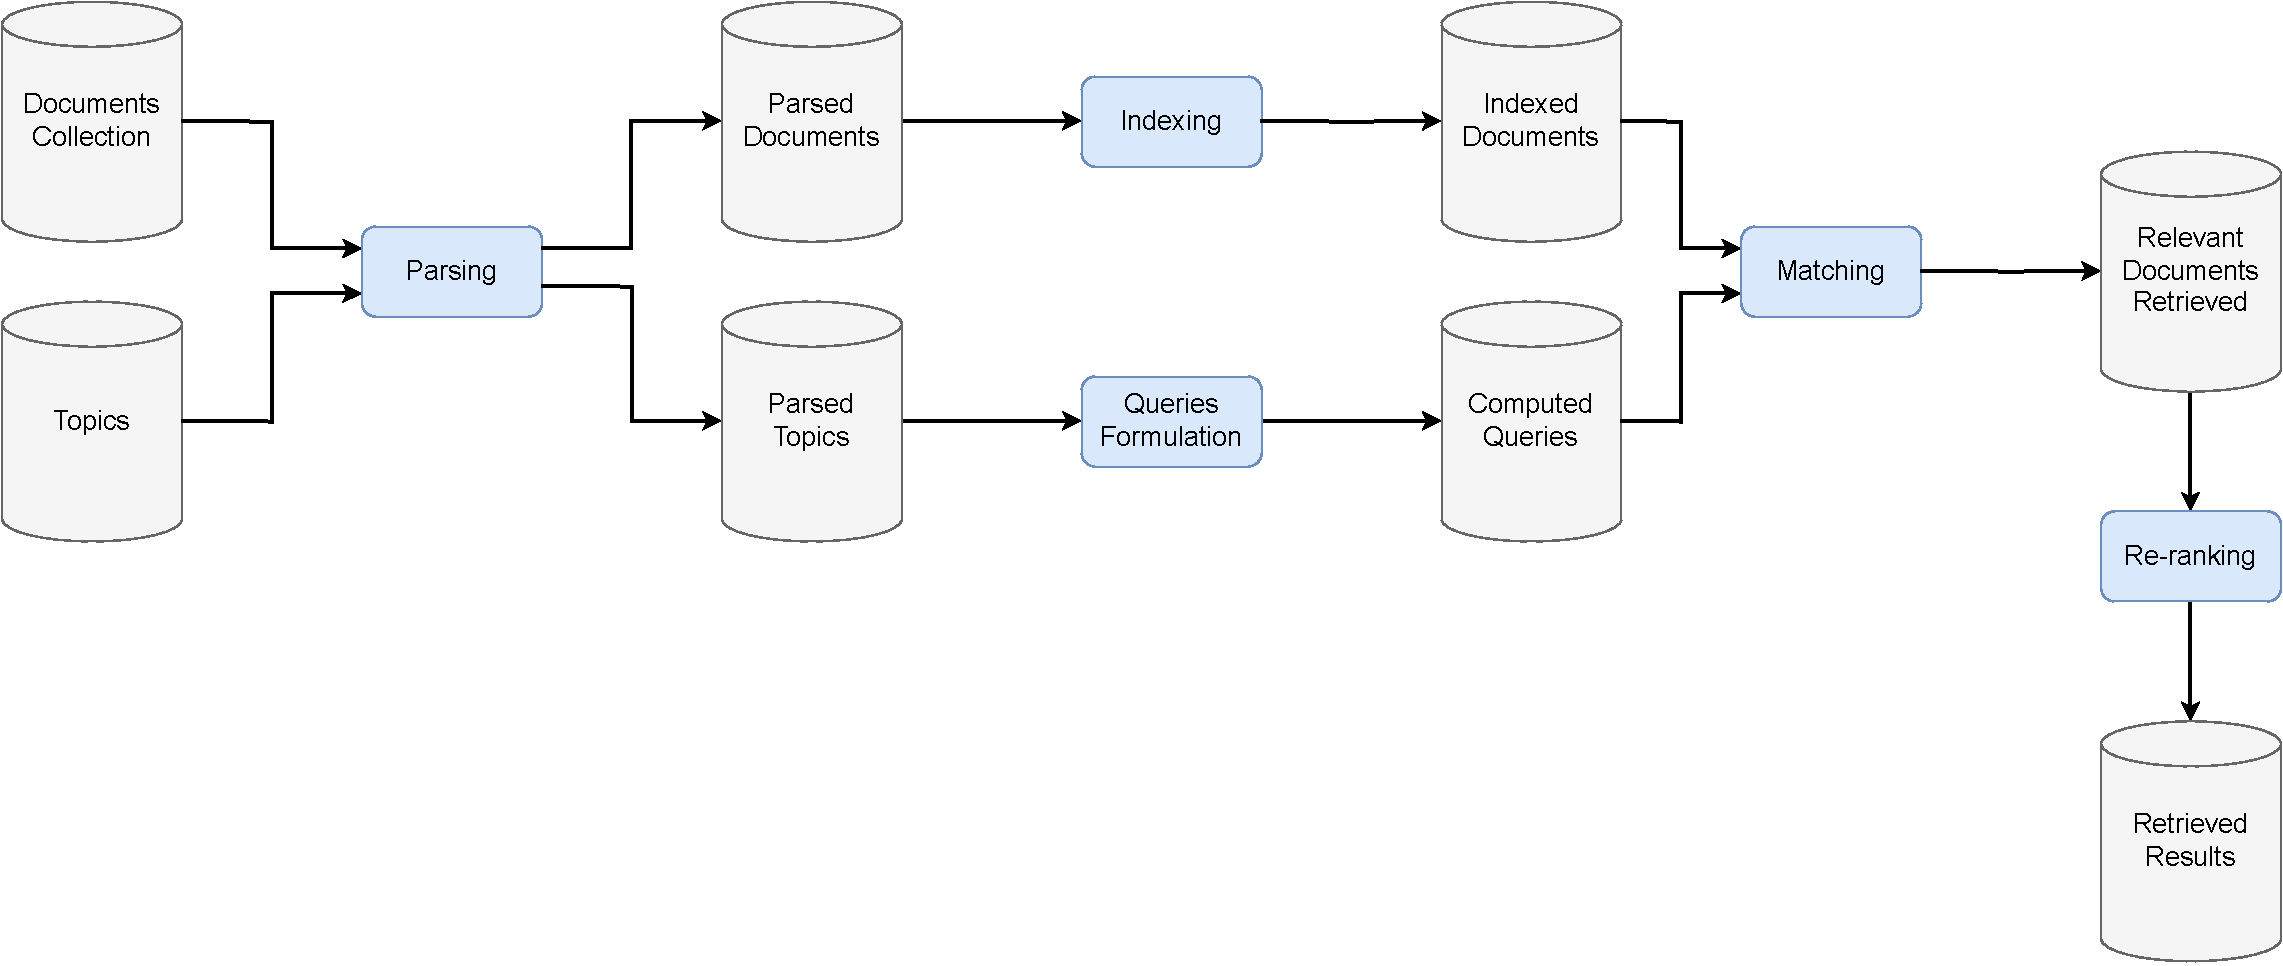
\includegraphics[width=\textwidth, height=\textheight, keepaspectratio]{figure/CLOSE_IR_Workflow (2).pdf}
    \caption{Workflow of the IR system implemented by \textit{CLOSE}.}
    \label{fig:CLOSE_IR_Workflow}
\end{figure}

\newpage
\enlargethispage{5\baselineskip}
\subsection{Class Diagram}

\begin{figure}[!h]
    \centering
    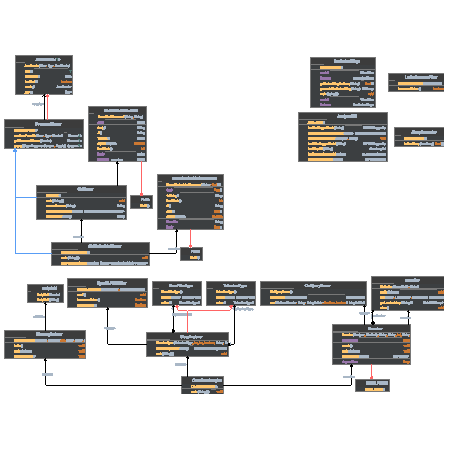
\includegraphics[height=0.7\textheight, angle =90, keepaspectratio]{figure/Classes_diagram_white_crop.pdf}
    \caption{Diagram of the classes implemented by \textit{CLOSE} \ac{IR} system}
    \label{fig:Classes_diagram_white}
\end{figure}
\clearpage
The class diagram of the system [\ref{fig:Classes_diagram_white}] retraces the Y model [\ref{fig:lucene_yModel}] of an IR system: in fact, it is possible to see it as an indexer class and a searcher class that is, in this order,
called by the main class \textit{CloseSearchEngine} of our system. The \textit{Analyzer} class is instantiated before all, as it is used both from the two main branches stated before. Here many other Lucene (and Solr for NLP filters trials) tools are instantiated, as long as this component
is responsible for analyzing tokens, and here most of our processing phase goes on: in particular, the tokenizer and the stemmer (and some NLP filters used in a trial).\\
The other connected component of the diagram is related to the parsing section: here, while walking on the file tree, the \textit{Indexer} uses this component to generate, from a JSON document, an actual Java object (\textit{ParsedTextDocument}) representing it with its fields.\\
The \textit{Searcher} class firstly parses the queries from the \ac{TREC} format in a Lucene \textit{QualityQuery} object, through our \textit{ClefQueryParser} class. It also instantiates the \textit{ReRanker}, responsible for the second-ranking phase.\\
Other utility classes are included but no longer used in our project.

\subsection{Parser} \label{parser_subsec}
As stated before, the documents in the collection provided by the \ac{CLEF} \textit{LongEval LAB 2023} \cite{cleflongeval} are essentially the corpus of web pages, to better represent the nature of a web test collection.
From this, the need for performing a pre-processing phase of parsing the documents before analyzing and indexing them arises.
In this phase, the documents are cleaned from all the residuals of codes not useful for our purposes. 
We first created an abstract class \textit{DocumentParser} and then extended it by implementing a custom \textit{ClefParser} class, which contains many functions for removing sundry types of noises that can be present in documents. 
This was the result of the trial and error approach we adopted for implementing this class:
\begin{itemize}
\item We started with our own read of a large statistical sample size of the documents in the collection to decide which types of noises needed to be removed.
\item Then we implemented the parser and ran it.
\item The results of the parsing were stored, and a sample of the parsed documents was analyzed to start this procedure again.
\end{itemize}

\begin{figure}[!h]
    \centering
    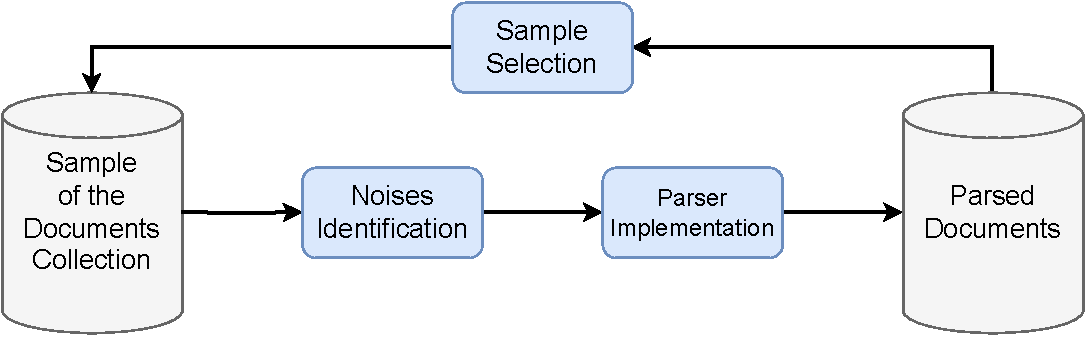
\includegraphics[width=0.8\linewidth]{figure/Parser_implementation_workflow.pdf}
    \caption{Workflow of the parser implementation.}
    \label{fig:Parser_implementation_workflow}
\end{figure}

\newpage
The types of noises we tried to remove are the following:
\begin{itemize}
\item \textit{JavaScript} scripts,
\item \textit{HTTP} and \textit{HTTPS} URIs,
\item \textit{HTML} tags and \textit{CSS} stylesheets,
\item \textit{XML} and \textit{JSON} codes,
\item Meta tags and document properties,
\item Navigation menus,
\item Advertisements,
\item Footers,
\item Social media handlers,
\item Hashtags and mentions.
\end{itemize}
The final decision about the type of noises to effectively remove for our runs was the most crucial part of this process. \\
For establishing this we used a trial \& error approach, and in the end, we decided to remove only the \textit{JavaScript} scripts and the \textit{HTTP} and \textit{HTTPS} URIs. Regarding \textit{URI}s, although these are usually important because they can contain valuable keywords, we noticed an improvement in \ac{MAP} of almost 0.5 points by just removing them. \\
We also identified some patterns of words and symbols to remove:
\begin{itemize}
\item Two words separated by an underscore, like \textit{word1\_word2}
\item Two words separated by a colon, like \textit{word1:word2}
\item Two words separated by a point, like ``\textit{word1.word2}''
\end{itemize}
We used \textit{Regular Expressions} \cite{regexdefinition} to identify and remove these patterns.  

The structure of the parsed document is defined in the \textit{ParsedTextDocument} class, and it is composed of just two fields, as provided by \ac{CLEF}:
\begin{enumerate}
\item \textit{id}: the identifier of the document,
\item \textit{body}: the (parsed) content of the document.
\end{enumerate}
Inside it, multiple controls about the validity and integrity of the parameters are performed, then an object of the class is instantiated.


\subsection{Analyzer} \label{analyzer_subsec}
The Analyzer is responsible for analyzing the extracted documents and preparing them for the Indexing and Searching phases.
It does so by combining a series of techniques of text processing such as tokenization, stemming, stopword removal, and many more.\\
We extended Apache Lucene's Analyzer abstract class \cite{luceneanalyzer} by creating a custom class \textit{CloseAnalyzer}, which is fully customizable by its parameters that can be chosen when creating an instance of the class.
This has been done because we tried different settings and approaches to maximize the results and kept all the possible variations as optional settings.
This \textit{CloseAnalyzer} is passed as a parameter and then used by the \textit{DirectoryIndexer} and by the \textit{Searcher}. \\
The constructor of \textit{CloseAnalyzer} accepts the following parameters:
\begin{itemize}
  \item \textbf{tokenizerType}: used to choose between three standard \textit{Lucene} tokenizers: \textit{WhitespaceTokenizer} \cite{lucenetokenizer}, \textit{LetterTokenizer} \cite{lucenelettertokenizer}, and \textit{StandardTokenizer} \cite{lucenestandardtokenizer}.

  \item \textbf{stemFilterType}: the possible choices for the stemming types are four standard \textit{Apache Solr} \cite{solr} filters: \textit{EnglishMinimalStemFilter} \cite{solrminimalstemfilter}, \textit{KStemFilter} \cite{solrkstemfilter}, \textit{PorterStemFilter} \cite{solrporterstemfilter}, and \textit{FrenchLightStemFilter} \cite{solrfrenchlightstemfilter}.
  We also tried using \textit{FrenchMinimalStemFilter} \cite{solrfrenchminimalstemfilter} and a custom filter called \textit{LovinsStemmerFilter} based on a LovinsStemmer \cite{lucenelovinsstemmer} implementation but decided to keep them commented as they didn't improve the results.

  \item \textbf{minLength} and \textbf{maxLength}: these are integers that simply specify the minimum and maximum length of a token, applying Lucene's \textit{LengthFilter} \cite{lucenelengthfilter}.

  \item \textbf{isEnglishPossessiveFilter}: specifies whether to use Lucene's \textit{EnglishPossessiveFilter} \cite{luceneenglishpossessivefilter} or not.
  Of course, this can be useful when operating with the English dataset.

  \item \textbf{stopFilterListName}: with this parameter, it's possible to insert the path of an eventual word stoplist \textit{.txt} file located in the \textit{resources} folder.
  To do this we use Lucene's \textit{StopFilter} \cite{lucenestopfilter} and a custom class called \textit{AnalyzerUtil} that uses a \textit{loadStopList} method to read and load all the stoplist words from the specified file.
  The stoplists we created are based on the standard ones but modified after inspecting the index with the \textit{Luke} \cite{luke} tool.
  We have lists of different lengths and different ones for French and English.

  \item \textbf{Character nGramFilterSize}: if specified, this parameter is used to define the size of the n-grams to be applied by Lucene's \textit{NGramTokenFilter} \cite{lucenengramtokenfilter}.

  \item \textbf{Word nGramFilterSize}: similar to the previous one, if used, this integer number indicates the shingle size to be applied by Lucene's \textit{ShingleFilter} \cite{luceneshinglefilter} that allows the creation of a combination of words.

  \item \textbf{useNLPFilter}: this boolean allows the use of Solr's \cite{solr} \textit{OpenNLPPPOSFilter} \cite{solropennlpposfilter} for Part-Of-Speech Tagging and of a custom class called \textit{OpenNLPNERFilter} for Named Entity Recognition.
  To load the \textit{.bin} models, which are located in the \textit{resources} folder, we use two methods from \textit{AnalyzerUtil}: \textit{loadPosTaggerModel} and \textit{loadNerTaggerModel}.

  \item \textbf{lemmatization}: specifies whether to use Solr's \textit{OpenNLPLemmatizerFilter} \cite{solropennlplemmafilter} by loading a \textit{.bin} model file in the \textit{resources} folder using AnalyzerUtil's \textit{loadLemmatizerModel} function.

  \item \textbf{frenchElisionFilter}: we applied this only when using the French dataset by adding Lucene's \textit{ElisionFilter} \cite{luceneelisionfilter} with an array of the following characters: 'l', 'd', 's', 't', 'n', 'm'.
\end{itemize}
On top of this, a \textit{LowerCaseFilter} \cite{lucenelowercasefilter} is always applied. \\
We also tried Lucene's \textit{ASCIIFoldingFilter} \cite{luceneasciifoldingfilter} and \textit{SynonymGraphFilter} \cite{lucenesynonymgraphfilter}.
For the second one, only for the French Dataset, we used a \textit{SynonymMap} \cite{lucenesynonymmap} based on a \textit{.txt} file containing French synonyms.
\newline
After different trials with different variations of the parameters, the following are options used with our \textit{CloseAnalyzer} implementation: we have opted for the French dataset and by doing so we have the \textit{StandardTokenizer}, 2 and 15 as minimum and maximum token length, we use \textit{frenchElisionFilter}, \textit{FrenchLightStemFilter}, and a list of 662 French words as a stoplist.
This stoplist has been built upon a popular French stoplist together with the most frequent stopwords in the collection.  
We didn't use any of the other parameters.
We utilized the Gson library to efficiently parse JSON files that contained query expansions. By leveraging Gson's capabilities, we were able to seamlessly convert the JSON data into Java objects, enabling effortless manipulation and integration of the query expansions into our application.


\subsection{Searcher} \label{searcher_subsec}
The purpose of the \textit{Searcher} is to search through the indexed documents to retrieve relevant information based on user queries after analyzing them and to
return a ranked list of documents that match the user’s information needs.
\newline
Our implementation does so by accepting the following parameters:
\begin{itemize}
  \item \textbf{analyzer}: in this case, an instance of \textit{CloseAnalyzer}.
  \item \textbf{similarity}: we decided to opt for the \textit{BM25Similarity} \cite{lucenebm25similarity} function with the parameters \textit{k1} and \textit{b} tuned at 1.2 and 0.90.
  \item \textbf{Run options}: there are parameters for the index path, the topics path, the run path and the run name, the number of the expected topic (in our case 50), and the maximum number of documents retrieved (in our case 1000).
  \item \textbf{reRankModel}: this is the type of model used to do a Re-Ranking on the retrieved documents. 
  In our case, we use a model called \textit{all-MiniLM-L6-v2} \cite{huggingfaceallminilml6v2}, explained in the following subsection. 
  If the parameter is set to null, no model is used and the documents are scored normally.
\end{itemize}

\newpage
\subsubsection{Query Expansion}
When running the search function, one of the first actions performed is to generate new queries from the original ones by query expansion \cite{wang2023}. \\
% For this task we have taken inspiration from the work of Shuai Wang \cite{wang2023}. 
We created a Python script that, given the \textit{*.trec} topic file, generates all the expanded terms for each query and stores everything in a \textit{.json} file called \textit{result}, containing all the expansions.
\newline
We use \textit{OpenAI's} \textit{Text completion} \cite{openaicompletionapi} endpoints to generate the expansions, we can use our need as a prompt and the model will generate the result. 
We used the \textit{davinci} model, which is the most powerful one, and we set the \textit{temperature} parameter to 0.6, which is the value that gives the best results.
\newline
The sample result for prompt 
\begin{center}
    \textit{``Expand the following query with {num\_expansions} related terms or phrases for information retrieval (search-engine): {query} and the result should be in array format without any numbers at first [expanded\_term1, expanded\_term2, ...]''}     
\end{center}
is:
\begin{table}[H]
    \begin{tabular}{|l|l|l|}
        \hline
        Query                 & text-davinci-002                                                                                                                                                                  & text-davinci-003                                                                                                                                                                    \\ \hline
        antivirus comparison & \begin{tabular}[c]{@{}l@{}}1. Antivirus software\\ 2. Antivirus protection\\ 3. Best antivirus\\ 4. Free antivirus\\ 5. Antivirus for Windows\\ 6. Antivirus for Mac\end{tabular} & \begin{tabular}[c]{@{}l@{}}1. Antivirus Reviews \\ 2. Antivirus Software \\ 3. Antivirus Protection \\ 4. Malware Protection \\ 5. Virus Scanner \\ 6. Online Security\end{tabular} \\ \hline
    \end{tabular}
    \label{tab:query_expansion}
\end{table}
The main difference between \textit{davinci-text-002} and \textit{davinci-text-003} is that the latter has been trained on a larger dataset, allowing it to generate more accurate results \cite{davincicomparison}.


\enlargethispage{2\baselineskip}
\subsubsection{Query Boosting}
Query boosting is a technique used to assign greater relevance to certain query terms or queries.\newline
We tried the following approach that seemed to improve the overall results: when building the queries in the search function of the \textit{Searcher} (\ref{searcher_subsec}), for each query, a \textit{BooleanQuery} \cite{lucenebooleanquery} is built in the following way: 
after getting the query expansions, each of them is added to the \textit{BooleanQuery} with the clause \textit{SHOULD} (meaning that at least one of them must be satisfied) and a main query is added with the clause \textit{MUST}, indicating that it must be satisfied. \\
This main query is boosted using Lucene's \textit{BoostQuery} \cite{luceneboostquery}, with a boost value tuned at 14.68 multiplied by the number of expansions. We got this value by a trial \& error approach we used to fine-tune this parameter.


\newpage
\enlargethispage{6\baselineskip}
\subsubsection{Document Re-Ranking}
Re-Ranking is the process of ranking documents retrieved by the search function of the \textit{Searcher} (\ref{searcher_subsec}). 
To accomplish this task, we utilized sentence transformers~\cite{sentence-transformers}, a Python framework known for its state-of-the-art sentence, text, and image embeddings. 
Various models were experimented with, and the one yielding the best results was identified as \textit{all-MiniLM-L6-v2}~\cite{huggingfaceallminilml6v2}. 
This particular model aims to train sentence embedding models using a self-supervised contrastive learning objective on vast sentence-level datasets, ultimately mapping sentences and paragraphs to a dense vector space of 384 dimensions.

To generate embeddings for both the documents and query retrieved by the search function, we loaded the \textit{all-MiniLM-L6-v2} model and instantiated a \textit{SentenceTransformer} object. 
To calculate similarity, we employed the widely used \textit{cosine similarity} formula, which computes the similarity between two vectors. The formula is defined as follows:

\begin{equation}
\text{similarity} = \frac{t \cdot d_i}{|t| |d_i|}\label{eq:similarity_equation}
\end{equation}

Here, $t$ represents the query vector, and $d_i$ denotes the vector of the $i$-th document.

Subsequently, we interpolated this similarity score with the BM25 score to improve the ranking of the documents. 
Among the different approaches we explored, the most successful one was as follows:


\begin{equation}
\text{rank} = \text{BM25\_score} \times \text{similarity} \label{eq:rank_equation}
\end{equation}

To visualize the re-ranking operation's effectiveness, we plotted the results for 50 sample queries, as depicted in Figure \ref{fig:re-ranking}.

\begin{figure}[!ht]
\centering
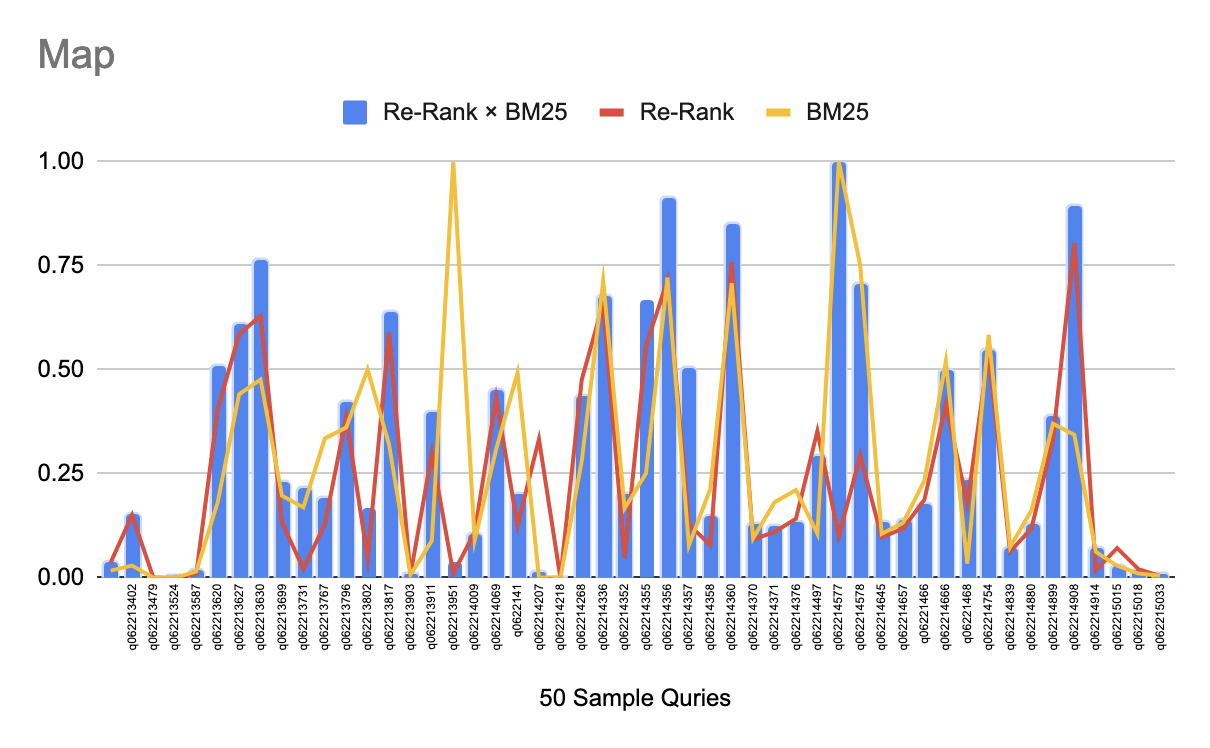
\includegraphics[scale=0.42, keepaspectratio]{figure/re-ranking}
\caption{Plot illustrating the re-ranking operation performed on 50 sample queries}
\label{fig:re-ranking}
\end{figure}

Finally, we sorted the documents based on the new rank and returned them.




% \enlargethispage{3\baselineskip}
\section{Experimental Setup}
\label{sec:setup}

\subsection{Collections}
We developed our model using a collection of 1,593,376 documents and 882 queries provided by \textit{Qwant} search engine, available at \url{https://lindat.mff.cuni.cz/repository/xmlui/handle/11234/1-5010}.
\newline
The collection contains information about user web searches and actual web pages corpora. The data was originally all in French but, for both queries and documents, an English translation is provided.


\subsection{Evaluation Measures}
To measure the effectiveness of our \ac{IR} system we used the \textit{trec\_eval} executable by testing it with the resulting runs produced by the model and its different configurations.
\newline
We tracked improvements of the following evaluation measures generated by \textit{trec\_eval}:
\begin{itemize}
	\item \textbf{num\textunderscore ret}: number of documents retrieved for a given query.
	\item \textbf{num\textunderscore rel}: number of relevant documents for a given query.
	\item \textbf{num \textunderscore rel\textunderscore ret}: number of relevant documents retrieved for a given query.
    \item \textbf{map}: Mean Average Precision, a measure of the average relevance of retrieved documents across all queries. Its range is in 0-1, where 1 indicates that all relevant documents are ranked at the top of the result list.
    \newline
    It's calculated as follows:
    \begin{equation*}
        MAP = \frac{1}{N} \sum_{i=1}^{N}AP_i
    \end{equation*}
    where $N$ is the total number of queries and $AP_i$ is the average precision of $query_i$ and calculated as:
    \begin{equation*}
        AP = \frac{1}{RD} \sum_{k=1}^{n}P(k)r(k)
    \end{equation*}
    with $RD$ the number of relevant documents for the query, $n$ the number of total documents, $P(k)$ the precision at $k$ and $r(k)$ the relevance of the $k$th retrieved document (0 if not relevant, 1 otherwise).
    \newline
    A high \ac{MAP} score indicates that the model effectively retrieves relevant documents for a wide range of queries.
    \item \textbf{rprec}: R-Precision is the precision score computed at the rank corresponding to the number of relevant documents for a given query.
    \item \textbf{p@5} and \textbf{p@10}: Precision at 5 and at 10 is the precision computed at the top 5 and 10 retrieved documents for a given query.
    They are calculated as follows:
    \begin{equation*}
        P(5) = \frac{1}{5} \sum_{k=1}^{5}r(k) \qquad ; \qquad P(10) = \frac{1}{10} \sum_{k=1}^{10}r(k)
    \end{equation*}
    with $r(k)$ the relevance of the $k$th document.
    \newline
    These two values can be useful to understand if the system retrieves relevant documents early in the result list, making it easier for the user to find the information needed.

\end{itemize}


\subsection{Git Repository}
The \textit{git} repository of the project can be found at
\url{https://bitbucket.org/upd-dei-stud-prj/seupd2223-close/src/master/} and it is organized as follows:
\dirtree{%
.1 \textbf{/}.
.2 code/.
.3 src/main/.
.4 java/it/unipd/dei/se/.
.5 analyzer.
.5 indexer.
.5 parser.
.5 searcher.
.5 utils   <-- ReRanker and array converter util.
.5 \textit{CloseSearchEngine.java}   <-- main class.
.4 resources   <-- word stoplists and models for NER and POS.
.3 python\textunderscore scripts   <-- python scripts, results for embeddings, ....
.3 \textit{pom.xml}.
.2 runs   <-- run files.
.2 results   <-- result files.
}


\subsection{System Hardware}
For the most time during the development of the system every member of the group ran the model on its own system, but after implementing the deep learning techniques we decided to switch and start running the tasks using GPU to improve time performances. \\
The following are the specifics of the machines used after switching to computing also with GPU:
\begin{itemize}
	\item CPU: Intel® Core™ i9-12900H 12th generation
	\item GPU: NVIDIA RTX™ A 2000 4GB GDDR6
	\item RAM: 16 GB SO-DIMM DDR5 4800MHz
	\item SSD: 512 GB M.2 2280 PCIe Gen4 TLC Opal
\end{itemize}
\begin{itemize}
	\item CPU: Ryzen 7 1700 overclocked at 3.8GHz
	\item GPU: RTX 3070 TI 8GB GDDR6X
	\item RAM: 16GB  DDR4 3000MHz
	\item SSD: Samsung evo 970 250GB
\end{itemize}




\pagebreak
\section{Results and Discussion}
\subsection{French}
\label{sec:results}

In this section we provide some of the most relevant results we got during the development phase.
We are considering five principal milestones that, within many different trials, led us to improve significantly our MAP score and the overall number of relevant documents actually retrieved.


    \begin{table}[h]
    \centering
    \begin{tabular}{ |l|c|c|c|c|c| }
        \hline
        metric & run1 & run2  & run3 & run4 &run 5 \\ \hline
        num\_q & 663 & 663 & 669 & 669 & 667 \\ \hline
        num\_ret & 654909 & 655684 & 658446 & 658347 & 657903 \\ \hline
        num\_rel & 2571 & 2571 & 2611 & 2611 & 2600 \\ \hline
        num\_rel\_ret & 1914 & 2084 & 2182 & 2191 & 2232 \\ \hline
        map & 0.1553 & 0.1875 & 0.2022 & 0.2029 & 0.2351 \\ \hline
        gm\_map & 0.0178 & 0.0348 & 0.046 & 0.0459 & 0.0629 \\ \hline
        Rprec & 0.1276 & 0.1571 & 0.1697 & 0.1628 & 0.2022 \\ \hline
        bpref & 0.3331 & 0.3626 & 0.3734 & 0.3761 & 0.3861 \\ \hline
        recip\_rank & 0.261 & 0.3037 & 0.3287 & 0.3281 & 0.3945 \\ \hline
        iprec\_at\_recall\_0.00 & 0.2775 & 0.3242 & 0.3499 & 0.3526 & 0.4182 \\ \hline
        iprec\_at\_recall\_0.10 & 0.2771 & 0.3236 & 0.3494 & 0.3523 & 0.4175 \\ \hline
        iprec\_at\_recall\_0.20 & 0.2577 & 0.3076 & 0.3324 & 0.337 & 0.3927 \\ \hline
        iprec\_at\_recall\_0.30 & 0.2113 & 0.2523 & 0.2679 & 0.2743 & 0.3236 \\ \hline
        iprec\_at\_recall\_0.40 & 0.1732 & 0.2152 & 0.2316 & 0.2323 & 0.2716 \\ \hline
        iprec\_at\_recall\_0.50 & 0.1614 & 0.2036 & 0.2193 & 0.2192 & 0.2533 \\ \hline
        iprec\_at\_recall\_0.60 & 0.133 & 0.1636 & 0.1786 & 0.1758 & 0.2014 \\ \hline
        iprec\_at\_recall\_0.70 & 0.1061 & 0.1281 & 0.1402 & 0.1402 & 0.1552 \\ \hline
        iprec\_at\_recall\_0.80 & 0.0892 & 0.1091 & 0.1178 & 0.12 & 0.1295 \\ \hline
        iprec\_at\_recall\_0.90 & 0.0742 & 0.0896 & 0.0956 & 0.0992 & 0.1033 \\ \hline
        iprec\_at\_recall\_1.00 & 0.0741 & 0.0895 & 0.0954 & 0.0986 & 0.1028 \\ \hline
        P\_5 & 0.1222 & 0.1475 & 0.1599 & 0.1614 & 0.1874 \\ \hline
        P\_10 & 0.0973 & 0.1192 & 0.1296 & 0.1312 & 0.1432 \\ \hline
        P\_15 & 0.0797 & 0.0965 & 0.1049 & 0.1068 & 0.1135 \\ \hline
        P\_20 & 0.0668 & 0.0805 & 0.088 & 0.0891 & 0.0935 \\ \hline
        P\_30 & 0.0519 & 0.0616 & 0.0661 & 0.0668 & 0.0703 \\ \hline
        P\_100 & 0.0206 & 0.0236 & 0.0256 & 0.0258 & 0.0268 \\ \hline
        P\_200 & 0.0116 & 0.0132 & 0.014 & 0.0141 & 0.0148 \\ \hline
        P\_500 & 0.0053 & 0.0059 & 0.0061 & 0.0061 & 0.0064 \\ \hline
        P\_1000 & 0.0029 & 0.0031 & 0.0033 & 0.0033 & 0.0033 \\ \hline
    \end{tabular}

\end{table}


\begin{figure}[h!]
    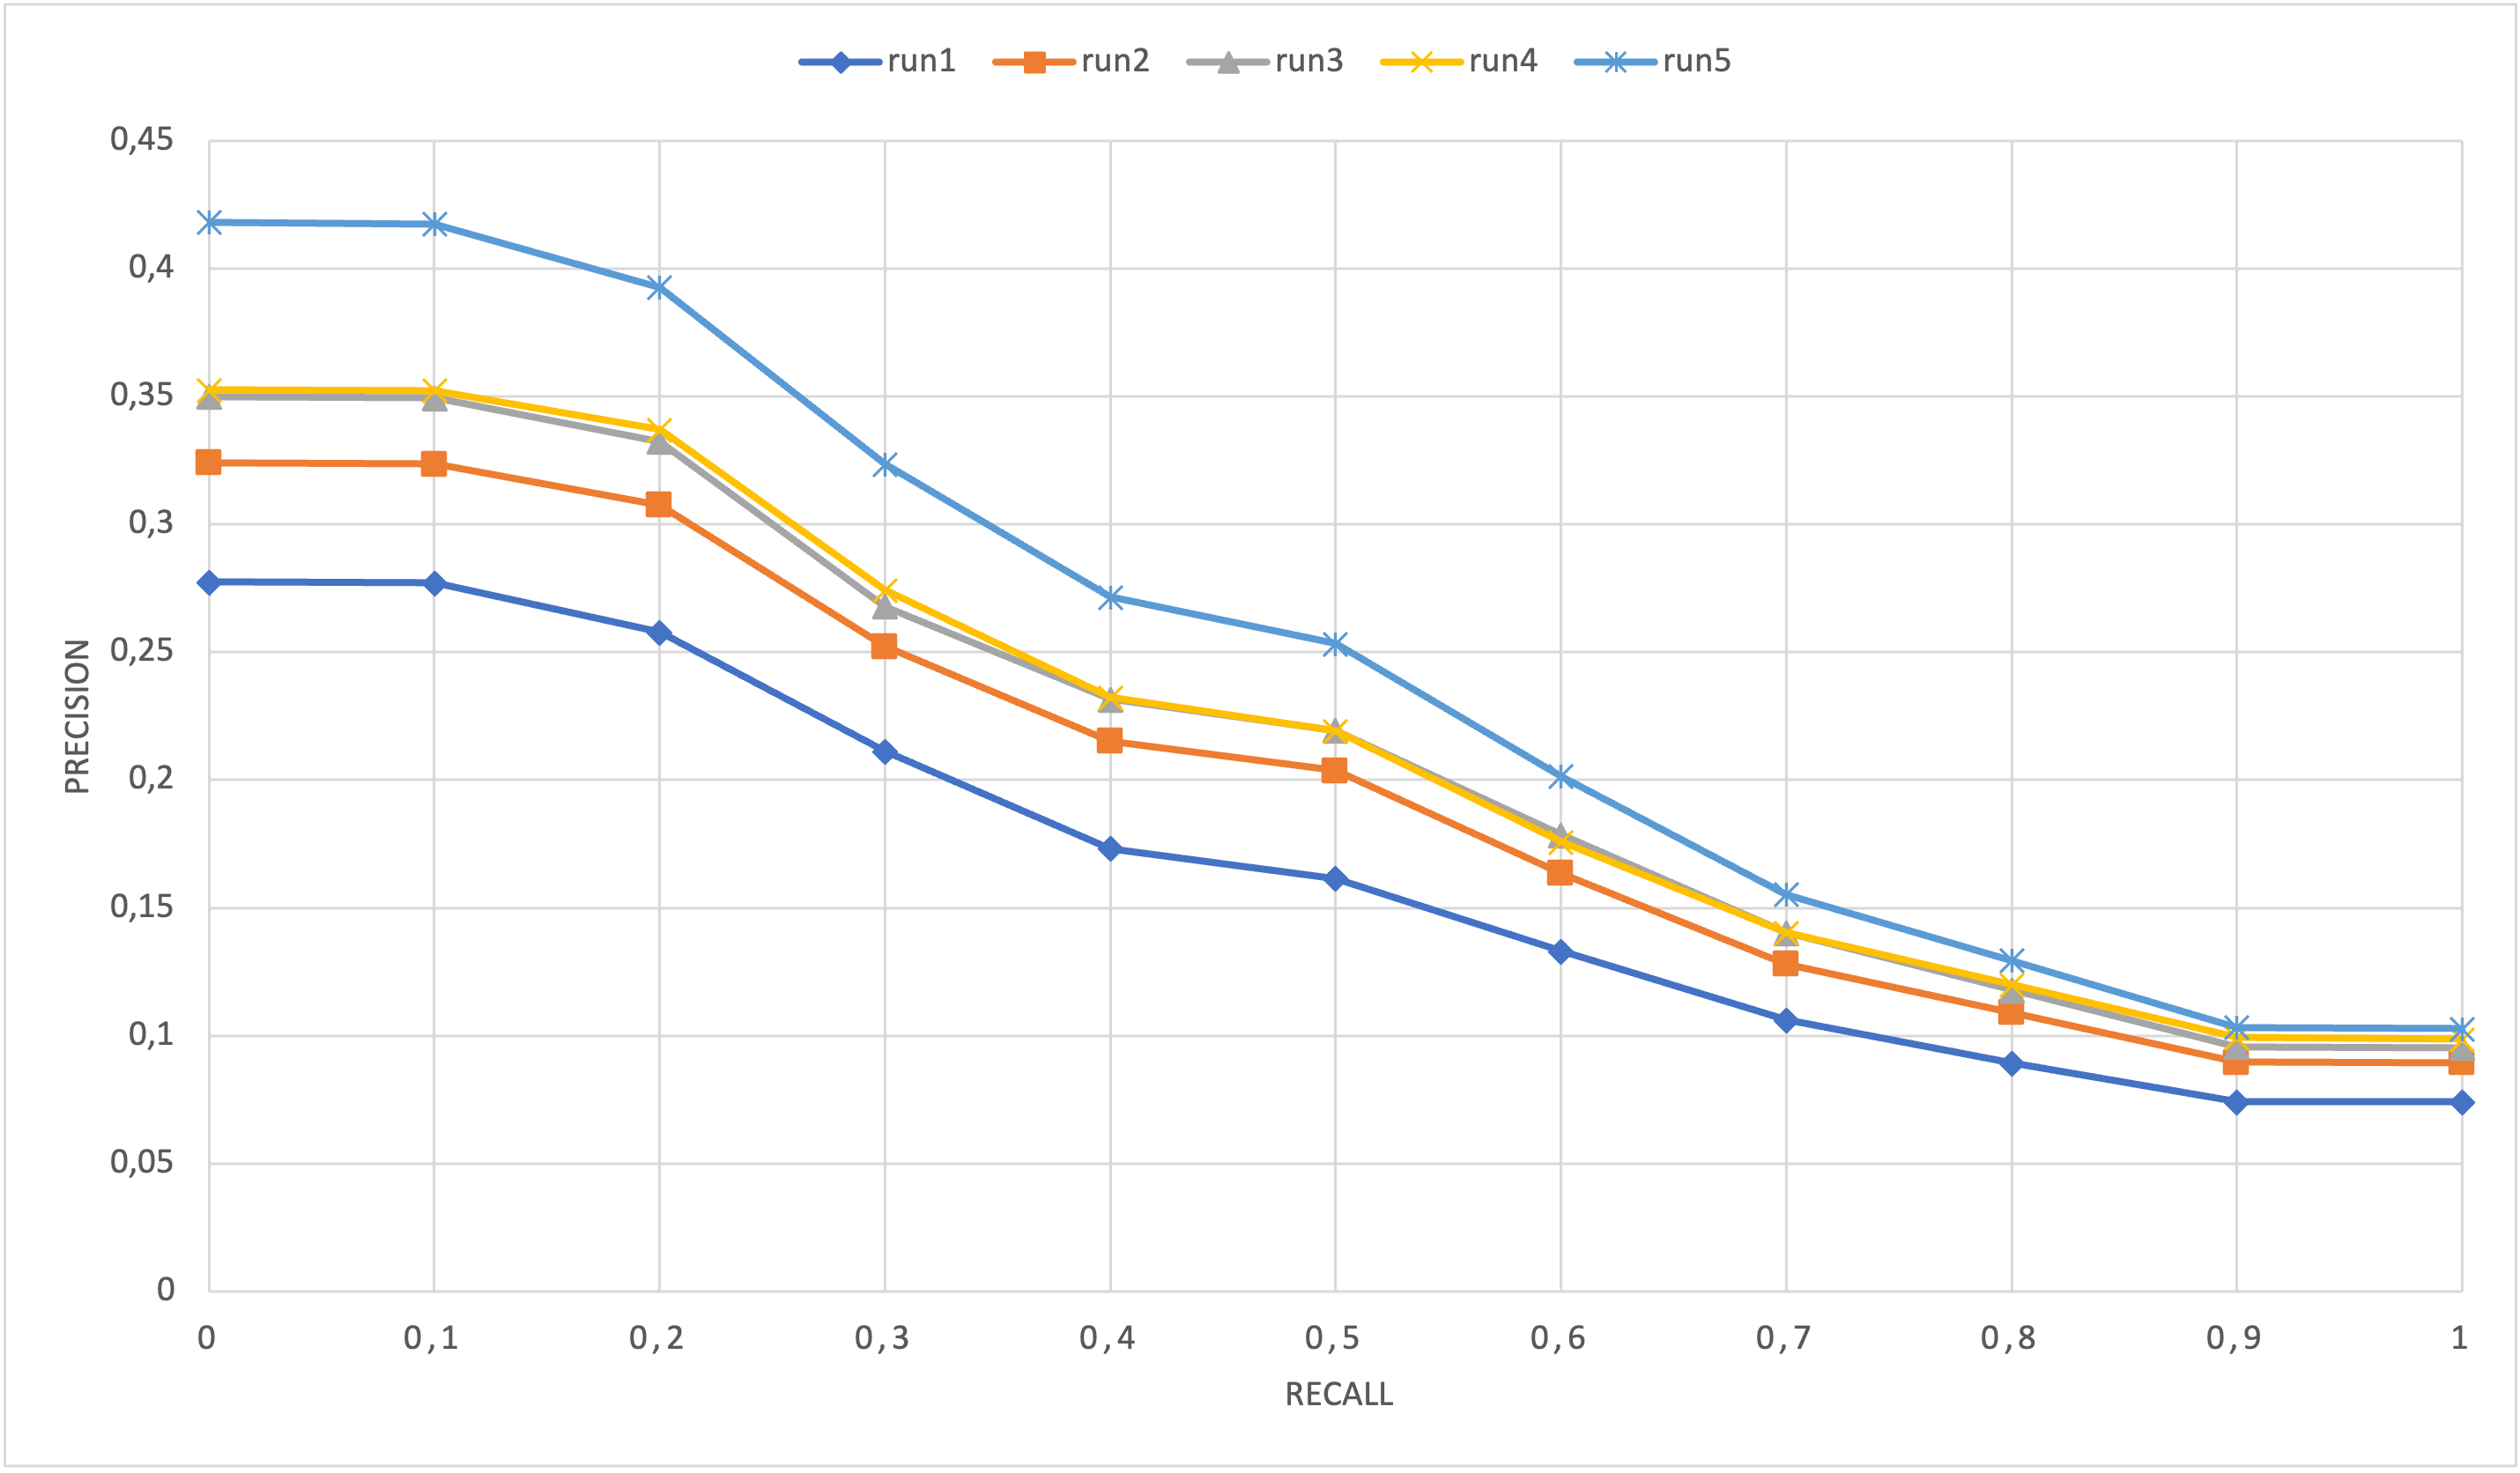
\includegraphics[width=\textwidth]{figure/rp_french.png}
    \caption{Recall and precision graph}
    \label{fig:rp_french}
\end{figure}

First of all, given that we were provided with two different version of the same document's \textit{corpora}, our first idea was to try with english version.\\ 
We noticed that the best combination of basic IR tools were to use the Porter stemmer, a lenght filter from 1 to 10, and a list of stopword composed by some standard terms and more from the top 600 extracted from the index.
The very first big milestone, that helped us to increment the MAP of around 3.5 points, was the JavaScript code parser, since we noticed by inspection that many documents were having code inside.\\
Always by inspecting some documents and queries, and also considering that the original collection was the french version (translated then in english), we observed that the translation was very poor: by switching to french
with just parsing the JS code and some other minor parsers, without even using an adequate stoplist and a correct stemmer for the french language, the MAP was increasing by 5 percentual points; 2 more points were achieved with
a stop list built for french in the same way we did for previously for english, the \textit{FrenchLightStemFilter} as stemmer, and moving the lenght filter from 2 to 15 (as french probabily usually has longer words).
We tried some NLP techniques for english, in particular using \textit{Part-Of-Speech} techniques, to see if there were improvements, and in case apply it to our main implementation for french with an appropriate model, but results 
were not interesting, and also the computing time were definitely too costly.
Another approach we tried and that carried an improvement was to use \textit{Query expansion}: we used some generative text models to expand our queries: we then decided to weight different query scores by boosting the original one linearly with respect to the number
of expansion used, and without boosting the expansion: this carried to us an extra MAP point.
We tried to combine different similarities rather than using the classic BM25Similarity: we tried to use the Lucene MultiSimilarity, that allows to combine equally the score of two or more similarity scores, but it does not allow to
tune the weights. Then, we tried to reimplement the MultiSimilarity class with tuning options, but results were always lower than the standard BM25Similarity. Some minor improvements came up by fine tuning the document-length
normalization \textit{b}, and the term frequency component \textit{k1} parameters of the BM25.
The last main implementation we did was to use some \textit{Reranking} techniques:  
Lastly, some minor addings were setted on the analyzer by implementing the Lucene ElisionFilter (for french), that aims to remove apostrophed articles and prepositions from tokens.

\subsection{English}
\begin{center}
    \begin{table}[h!]
    \begin{tabular}{ |l|c|c|c|c| } 
        \hline
        metrics & run1 & run2 & run3 & run4 \\ \hline
        num\_q & 657.0 & 657.0 & 667.0 & 665.0 \\ \hline
        num\_ret & 646525.0 & 646607.0 & 653936.0 & 653361.0 \\ \hline
        num\_rel & 2550.0 & 2550.0 & 2605.0 & 2594.0 \\ \hline
        num\_rel\_ret & 1772.0 & 1824.0 & 1886.0 & 1884.0 \\ \hline
        map & 0.1307 & 0.1377 & 0.1464 & 0.1875 \\ \hline
        gm\_map & 0.0117 & 0.0146 & 0.017 & 0.0261 \\ \hline
        Rprec & 0.1041 & 0.1107 & 0.1199 & 0.16 \\ \hline
        bpref & 0.3142 & 0.3223 & 0.3275 & 0.3481 \\ \hline
        recip\_rank & 0.2436 & 0.2594 & 0.2731 & 0.3369 \\ \hline
        iprec\_at\_recall\_0.00 & 0.2553 & 0.2719 & 0.2861 & 0.3552 \\ \hline
        iprec\_at\_recall\_0.10 & 0.2553 & 0.2706 & 0.2853 & 0.354 \\ \hline
        iprec\_at\_recall\_0.20 & 0.2387 & 0.2524 & 0.2668 & 0.3305 \\ \hline
        iprec\_at\_recall\_0.30 & 0.1854 & 0.1913 & 0.2002 & 0.2619 \\ \hline
        iprec\_at\_recall\_0.40 & 0.1441 & 0.1508 & 0.1589 & 0.2142 \\ \hline
        iprec\_at\_recall\_0.50 & 0.1302 & 0.1359 & 0.1436 & 0.1946 \\ \hline
        iprec\_at\_recall\_0.60 & 0.0965 & 0.1026 & 0.1101 & 0.147 \\ \hline
        iprec\_at\_recall\_0.70 & 0.0746 & 0.0792 & 0.0873 & 0.1122 \\ \hline
        iprec\_at\_recall\_0.80 & 0.0628 & 0.0677 & 0.0752 & 0.0929 \\ \hline
        iprec\_at\_recall\_0.90 & 0.0526 & 0.0573 & 0.0616 & 0.0754 \\ \hline
        iprec\_at\_recall\_1.00 & 0.0525 & 0.0572 & 0.0615 & 0.0751 \\ \hline
        P\_5 & 0.1056 & 0.1102 & 0.1193 & 0.1504 \\ \hline
        P\_10 & 0.0848 & 0.0893 & 0.0954 & 0.1167 \\ \hline
        P\_15 & 0.0698 & 0.0727 & 0.078 & 0.0918 \\ \hline
        P\_20 & 0.0598 & 0.0621 & 0.0661 & 0.0769 \\ \hline
        P\_30 & 0.0469 & 0.0491 & 0.0515 & 0.058 \\ \hline
        P\_100 & 0.0186 & 0.0193 & 0.02 & 0.0225 \\ \hline
        P\_200 & 0.0106 & 0.011 & 0.0113 & 0.0124 \\ \hline
        P\_500 & 0.0049 & 0.0051 & 0.0052 & 0.0055 \\ \hline
        P\_1000 & 0.0027 & 0.0028 & 0.0028 & 0.0028 \\ \hline
    \end{tabular}
    \end{table}
\end{center}



\begin{figure}[h!]
    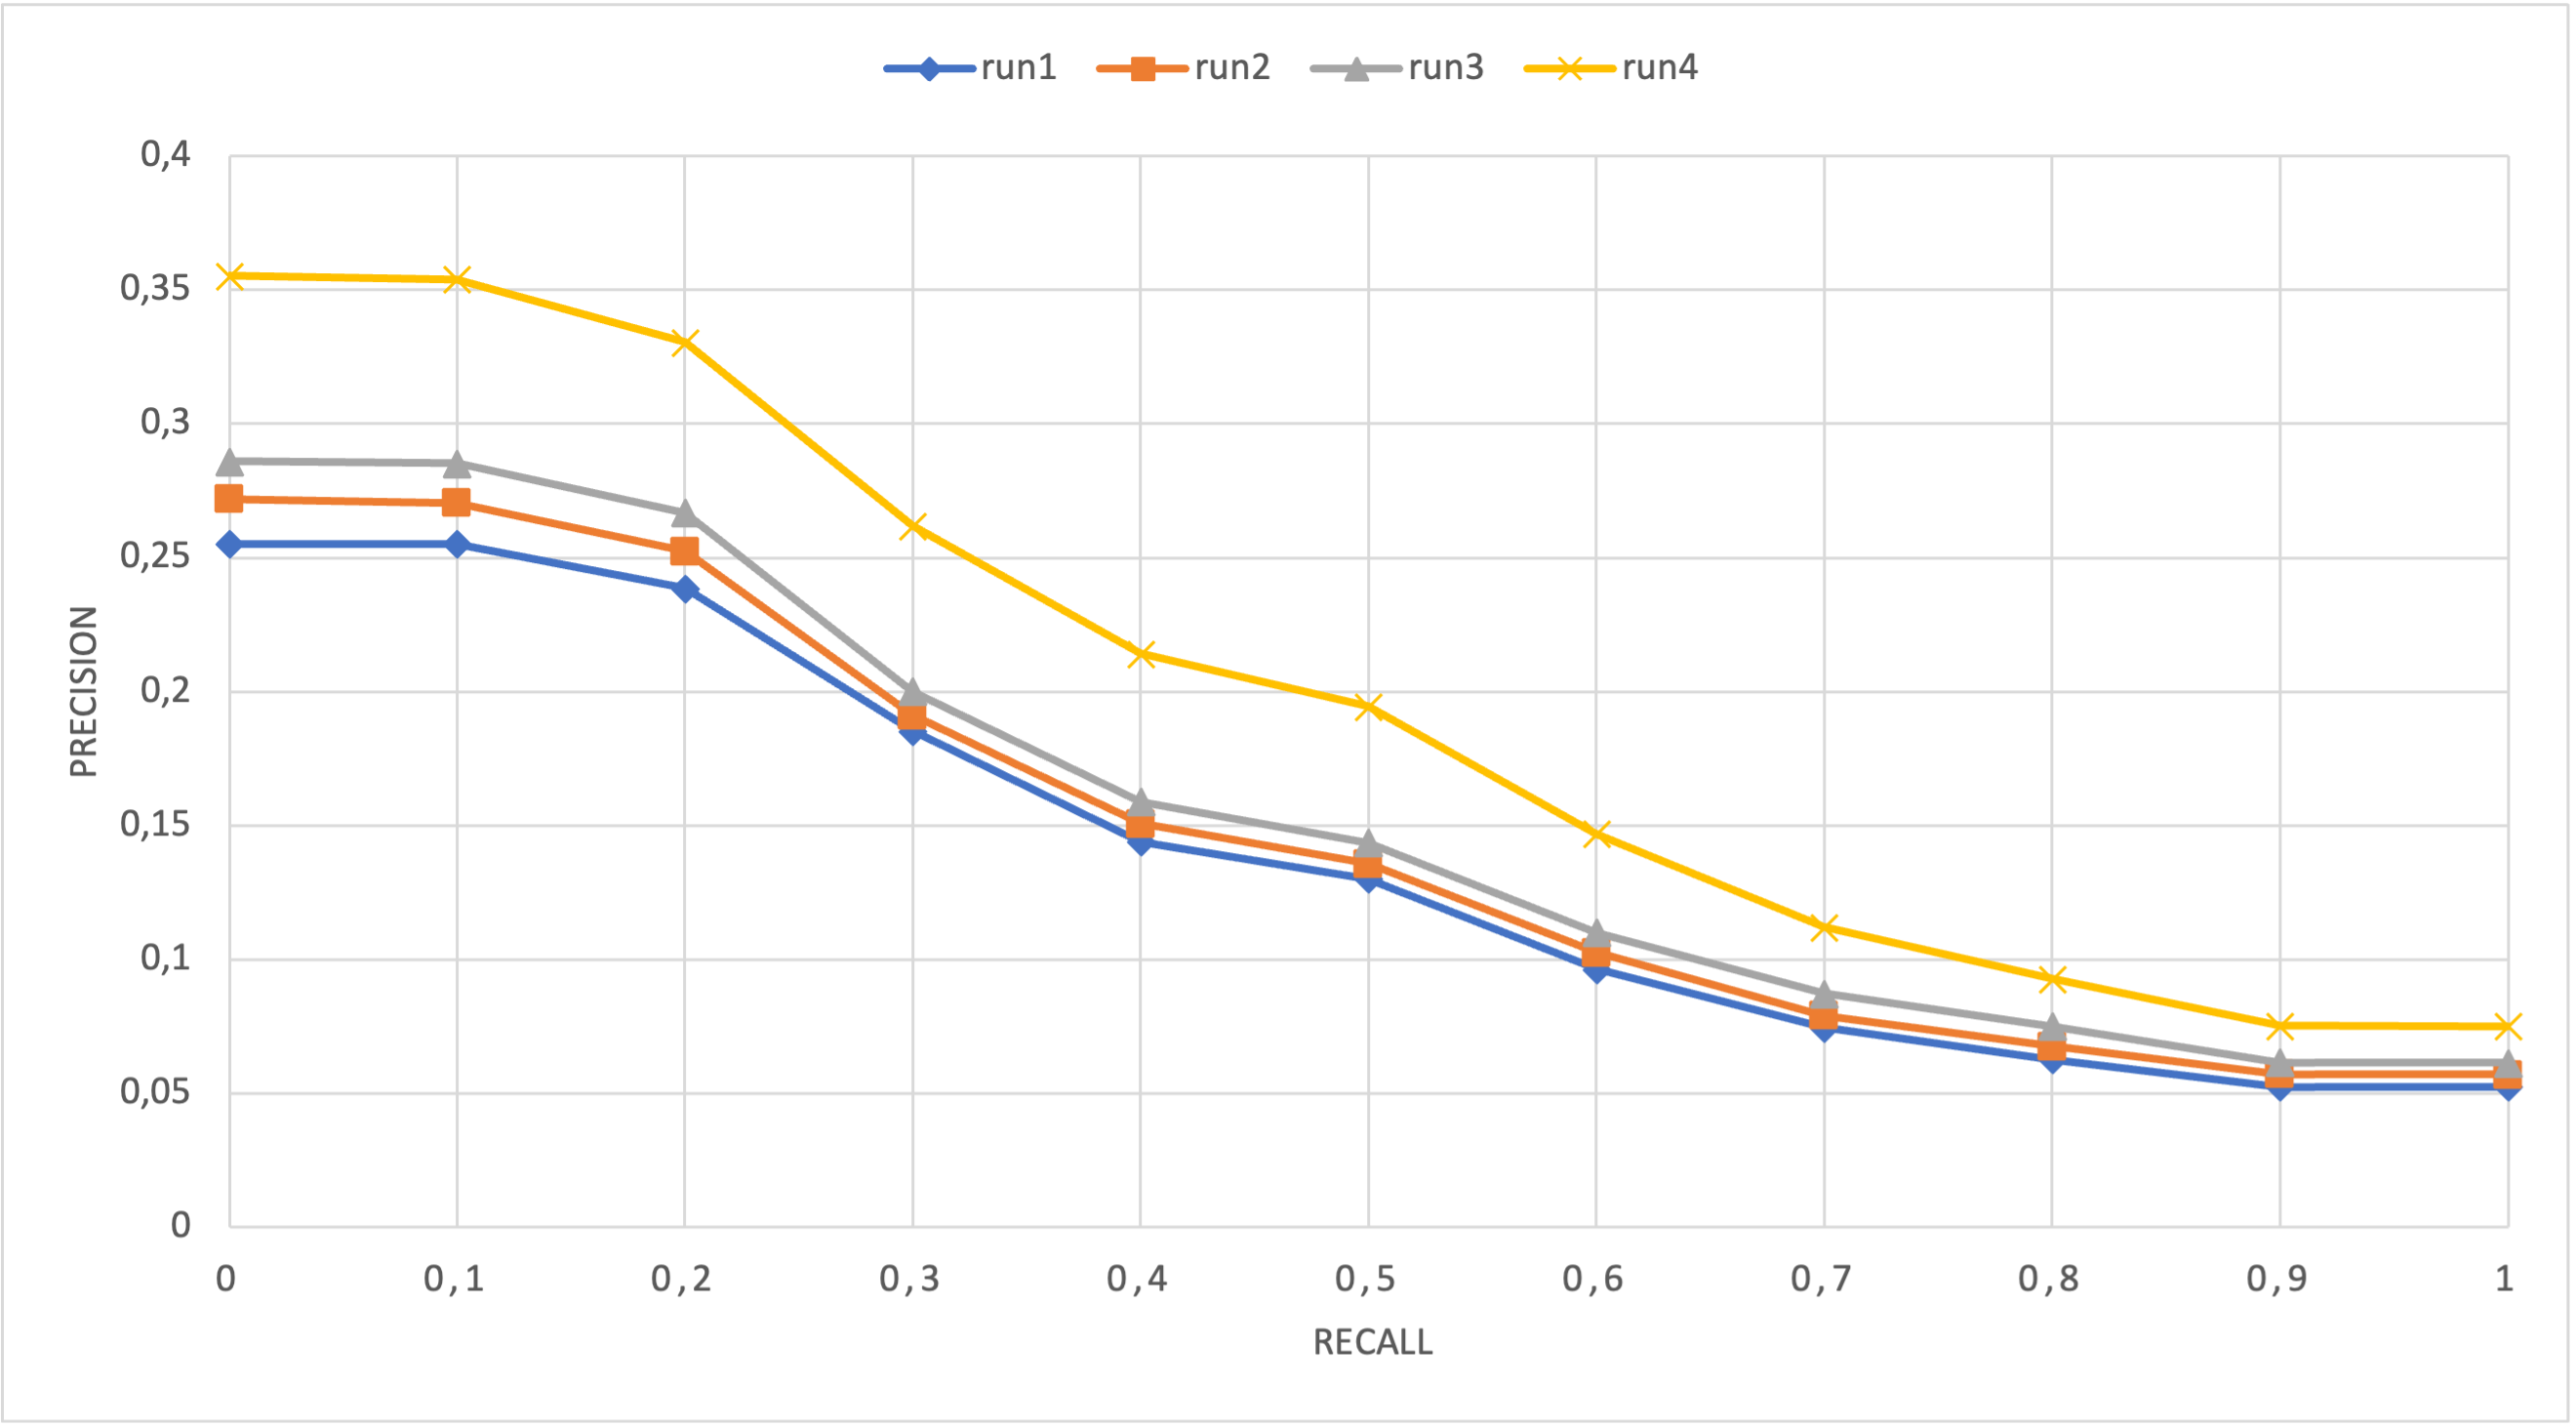
\includegraphics[width=\textwidth]{figure/rp_eng.png}
    \caption{Recall and precision graph}
    \label{fig:rp_english}
  \end{figure}


\section{Conclusions and Future Work}
\label{sec:conclusion}
 
In this work, we presented our approach to the \ac{CLEF} \textit{Long Eval LAB 2022} task, which aimed to develop an effective and efficient search engine for web documents. \\
Our approach consisted of using a combination of different techniques, including query expansion, re-ranking, and the use of large language models such as \textit{ChatGPT} and \textit{SBERT}. \\
Our experiments showed that our approach achieved good results in terms of effectiveness and efficiency, outperforming the baseline system provided by \ac{CLEF}. Specifically, we found that combining two different scores in the re-ranking phase led to significant improvements in the retrieval performance. Moreover, we identified several areas for future work that could further improve the effectiveness and efficiency of our approach. \\
One possible direction for future work is to find better ways to combine scores or add other scores to the re-ranking phase. We plan to explore different combinations of scores and investigate the use of other large language models, such as other available \textit{BERT} models trained, or to train some specifically for this task. \\
Another area for future work is to find better prompts \cite{wang2023chatgpt} to use in \textit{ChatGPT} for improving query expansion. We also plan to investigate the use of other \ac{LLM} techniques for query expansion. \\
We also want to explore ways to increase the similarity in \textit{SBERT}~\cite{reimers-2019-sentence-bert}, to increase the number of relevant documents found in the re-ranking phase. One possible approach is to fine-tune the \textit{SBERT}~\cite{reimers-2019-sentence-bert} model on our specific task. \\
Another direction for future work is to index documents as vectors and use them directly, instead of calculating them in re-ranking. This trade-off would result in the loss of one of the scores, but it would increase the re-ranking speed. \\
Finally, we plan to use links inside documents to extract details that may improve the searching results. We may try to find keywords in the URL path and use them to find their domain authority and take this aspect into account in the score computation.





%% Define the bibliography file to be used
\bibliography{bibliography,proceedings}

\acrodef{3G}[3G]{Third Generation Mobile System}
\acrodef{5S}[5S]{Streams, Structures, Spaces, Scenarios, Societies}
\acrodef{AA}[AA]{Active Agreements}
\acrodef{AAAI}[AAAI]{Association for the Advancement of Artificial Intelligence}
\acrodef{AAL}[AAL]{Annotation Abstraction Layer}
\acrodef{AAM}[AAM]{Automatic Annotation Manager}
\acrodef{AAP}[AAP]{Average Average Precision}
\acrodef{ACLIA}[ACLIA]{Advanced Cross-Lingual Information Access}
\acrodef{ACM}[ACM]{Association for Computing Machinery}
\acrodef{AD}[AD]{Active Disagreements}
\acrodef{ADSL}[ADSL]{Asymmetric Digital Subscriber Line}
\acrodef{ADUI}[ADUI]{ADministrator User Interface}
\acrodef{AIP}[AIP]{Archival Information Package}
\acrodef{AJAX}[AJAX]{Asynchronous JavaScript Technology and \acs{XML}}
\acrodef{ALU}[ALU]{Aritmetic-Logic Unit}
\acrodef{AMUSID}[AMUSID]{Adaptive MUSeological IDentity-service}
\acrodef{ANOVA}[ANOVA]{ANalysis Of VAriance}
\acrodef{ANSI}[ANSI]{American National Standards Institute}
\acrodef{AP}[AP]{Average Precision}
\acrodef{APC}[APC]{AP Correlation}
\acrodef{API}[API]{Application Program Interface}
\acrodef{AR}[AR]{Address Register}
\acrodef{AS}[AS]{Annotation Service}
\acrodef{ASAP}[ASAP]{Adaptable Software Architecture Performance}
\acrodef{ASI}[ASI]{Annotation Service Integrator}
\acrodef{ASL}[ASL]{Achieved Significance Level}
\acrodef{ASM}[ASM]{Annotation Storing Manager}
\acrodef{ASR}[ASR]{Automatic Speech Recognition}
\acrodef{ASUI}[ASUI]{ASsessor User Interface}
\acrodef{ATIM}[ATIM]{Annotation Textual Indexing Manager}
\acrodef{AUC}[AUC]{Area Under the ROC Curve}
\acrodef{AUI}[AUI]{Administrative User Interface}
\acrodef{AWARE}[AWARE]{Assessor-driven Weighted Averages for Retrieval Evaluation}
\acrodef{BANKS-I}[BANKS-I]{Browsing ANd Keyword Searching I}
\acrodef{BANKS-II}[BANKS-II]{Browsing ANd Keyword Searching II}
\acrodef{BH}[BH]{Benjamini-Hochberg}
\acrodef{bpref}[bpref]{Binary Preference}
\acrodef{BNF}[BNF]{Backus and Naur Form}
\acrodef{BPM}[BPM]{Bejeweled Player Model}
\acrodef{BRICKS}[BRICKS]{Building Resources for Integrated Cultural Knowledge Services}
\acrodef{CAN}[CAN]{Content Addressable Netword}
\acrodef{CAS}[CAS]{Content-And-Structure}
\acrodef{CBSD}[CBSD]{Component-Based Software Developlement}
\acrodef{CBSE}[CBSE]{Component-Based Software Engineering}
\acrodef{CB-SPE}[CB-SPE]{Component-Based \acs{SPE}}
\acrodef{CD}[CD]{Collaboration Diagram}
\acrodef{CD}[CD]{Compact Disk}
\acrodef{CDF}[CDF]{Cumulative Density Function}
\acrodef{CENL}[CENL]{Conference of European National Librarians}
\acrodef{CIDOC CRM}[CIDOC CRM]{CIDOC Conceptual Reference Model}
\acrodef{CIR}[CIR]{Current Instruction Register}
\acrodef{CIRCO}[CIRCO]{Coordinated Information Retrieval Components Orchestration}
\acrodef{CG}[CG]{Cumulated Gain}
\acrodef{CL}[CL]{Curriculum Learning}
\acrodef{CL-ESA}[CL-ESA]{Cross-Lingual Explicit Semantic Analysis}
\acrodef{CLAIRE}[CLAIRE]{Combinatorial visuaL Analytics system for Information Retrieval Evaluation}
\acrodef{CLEF1}[CLEF]{Cross-Language Evaluation Forum}
\acrodef{CLEF}[CLEF]{Conference and Labs of the Evaluation Forum}
\acrodef{CLIR}[CLIR]{Cross Language Information Retrieval}
\acrodef{CM}[CM]{Continuation Methods}
\acrodef{CMS}[CMS]{Content Management System}
\acrodef{CMT}[CMT]{Campaign Management Tool}
\acrodef{CNR}[CNR]{Italian National Council of Research}
\acrodef{CO}[CO]{Content-Only}
\acrodef{COD}[COD]{Code On Demand}
\acrodef{CODATA}[CODATA]{Committee on Data for Science and Technology}
\acrodef{COLLATE}[COLLATE]{Collaboratory for Annotation Indexing and Retrieval of Digitized Historical Archive Material}
\acrodef{CP}[CP]{Characteristic Pattern}
\acrodef{CPE}[CPE]{Control Processor Element}
\acrodef{CPU}[CPU]{Central Processing Unit}
\acrodef{CQL}[CQL]{Contextual Query Language}
\acrodef{CRP}[CRP]{Cumulated Relative Position}
\acrodef{CRUD}[CRUD]{Create--Read--Update--Delete}
\acrodef{CS}[CS]{Characteristic Structure}
\acrodef{CSM}[CSM]{Campaign Storing Manager}
\acrodef{CSS}[CSS]{Cascading Style Sheets}
\acrodef{CTR}[CTR]{Click-Through Rate}
\acrodef{CU}[CU]{Control Unit}
\acrodef{CUI}[CUI]{Client User Interface}
\acrodef{CV}[CV]{Cross-Validation}
\acrodef{DAFFODIL}[DAFFODIL]{Distributed Agents for User-Friendly Access of Digital Libraries}
\acrodef{DAO}[DAO]{Data Access Object}
\acrodef{DARE}[DARE]{Drawing Adequate REpresentations}
\acrodef{DARPA}[DARPA]{Defense Advanced Research Projects Agency}
\acrodef{DAS}[DAS]{Distributed Annotation System}
\acrodef{DB}[DB]{DataBase}
\acrodef{DBMS}[DBMS]{DataBase Management System}
\acrodef{DC}[DC]{Dublin Core}
\acrodef{DCG}[DCG]{Discounted Cumulated Gain}
\acrodef{DCMI}[DCMI]{Dublin Core Metadata Initiative}
\acrodef{DCV}[DCV]{Document Cut--off Value}
\acrodef{DD}[DD]{Deployment Diagram}
\acrodef{DDC}[DDC]{Dewey Decimal Classification}
\acrodef{DDS}[DDS]{Direct Data Structure}
\acrodef{DF}[DF]{Degrees of Freedom}
\acrodef{DFI}[DFI]{Divergence From Independence}
\acrodef{DFR}[DFR]{Divergence From Randomness}
\acrodef{DHT}[DHT]{Distributed Hash Table}
\acrodef{DI}[DI]{Digital Image}
\acrodef{DIKW}[DIKW]{Data, Information, Knowledge, Wisdom}
\acrodef{DIL}[DIL]{\acs{DIRECT} Integration Layer}
\acrodef{DiLAS}[DiLAS]{Digital Library Annotation Service}
\acrodef{DIRECT}[DIRECT]{Distributed Information Retrieval Evaluation Campaign Tool}
\acrodef{DKMS}[DKMS]{Data and Knowledge Management System}
\acrodef{DL}[DL]{Digital Library}
\acrodefplural{DL}[DL]{Digital Libraries}
\acrodef{DLMS}[DLMS]{Digital Library Management System}
\acrodef{DLOG}[DL]{Description Logics}
\acrodef{DLS}[DLS]{Digital Library System}
\acrodef{DLSS}[DLSS]{Digital Library Service System}
\acrodef{DM}[DM]{Data Mining}
\acrodef{DO}[DO]{Digital Object}
\acrodef{DOI}[DOI]{Digital Object Identifier}
\acrodef{DOM}[DOM]{Document Object Model}
\acrodef{DoMDL}[DoMDL]{Document Model for Digital Libraries}
\acrodef{DP}[DP]{Discriminative Power}
\acrodef{DPBF}[DPBF]{Dynamic Programming Best-First}
\acrodef{DR}[DR]{Data Register}
\acrodef{DRIVER}[DRIVER]{Digital Repository Infrastructure Vision for European Research}
\acrodef{DTD}[DTD]{Document Type Definition}
\acrodef{DVD}[DVD]{Digital Versatile Disk}
\acrodef{EAC-CPF}[EAC-CPF]{Encoded Archival Context for Corporate Bodies, Persons, and Families}
\acrodef{EAD}[EAD]{Encoded Archival Description}
\acrodef{EAN}[EAN]{International Article Number}
\acrodef{EBU}[EBU]{Expected Browsing Utility}
\acrodef{ECD}[ECD]{Enhanced Contenty Delivery}
\acrodef{ECDL}[ECDL]{European Conference on Research and Advanced Technology for Digital Libraries}
\acrodef{EDM}[EDM]{Europeana Data Model}
\acrodef{EG}[EG]{Execution Graph}
\acrodef{ELDA}[ELDA]{Evaluation and Language resources Distribution Agency}
\acrodef{ELRA}[ELRA]{European Language Resources Association}
\acrodef{EM}[EM]{Expectation Maximization}
\acrodef{EMMA}[EMMA]{Extensible MultiModal Annotation}
\acrodef{EPROM}[EPROM]{Erasable Programmable \acs{ROM}}
\acrodef{EQNM}[EQNM]{Extended Queueing Network Model}
\acrodef{ER}[ER]{Entity--Relationship}
\acrodef{ERR}[ERR]{Expected Reciprocal Rank}
\acrodef{ERS}[ERS]{Empirical Relational System}
\acrodef{ESA}[ESA]{Explicit Semantic Analysis}
\acrodef{ESL}[ESL]{Expected Search Length}
\acrodef{ETL}[ETL]{Extract-Transform-Load}
\acrodef{FAST}[FAST]{Flexible Annotation Service Tool}
\acrodef{FDR}[FDR]{False Discovery Rate}
\acrodef{FIFO}[FIFO]{First-In / First-Out}
\acrodef{FIRE}[FIRE]{Forum for Information Retrieval Evaluation}
\acrodef{FN}[FN]{False Negative}
\acrodef{FNR}[FNR]{False Negative Rate}
\acrodef{FOAF}[FOAF]{Friend of a Friend}
\acrodef{FORESEE}[FORESEE]{FOod REcommentation sErvER}
\acrodef{FP}[FP]{False Positive}
\acrodef{FPR}[FPR]{False Positive Rate}
\acrodef{FWER}[FWER]{Family-wise Error Rate}
\acrodef{GIF}[GIF]{Graphics Interchange Format}
\acrodef{GIR}[GIR]{Geografic Information Retrieval}
\acrodef{GAP}[GAP]{Graded Average Precision}
\acrodef{GLM}[GLM]{General Linear Model}
\acrodef{GLMM}[GLMM]{General Linear Mixed Model}
\acrodef{GMAP}[GMAP]{Geometric Mean Average Precision}
\acrodef{GoP}[GoP]{Grid of Points}
\acrodef{GPRS}[GPRS]{General Packet Radio Service}
\acrodef{gP}[gP]{Generalized Precision}
\acrodef{gR}[gR]{Generalized Recall}
\acrodef{gRBP}[gRBP]{Graded Rank-Biased Precision}
\acrodef{GT}[GT]{Generalizability Theory}
\acrodef{GTIN}[GTIN]{Global Trade Item Number}
\acrodef{GUI}[GUI]{Graphical User Interface}
\acrodef{GW}[GW]{Gateway}
\acrodef{HCI}[HCI]{Human Computer Interaction}
\acrodef{HDS}[HDS]{Hybrid Data Structure}
\acrodef{HIR}[HIR]{Hypertext Information Retrieval}
\acrodef{HIT}[HIT]{Human Intelligent Task}
\acrodef{HITS}[HITS]{Hyperlink-Induced Topic Search}
\acrodef{HMM}[HMM]{Hidden Markov Model}
\acrodef{HTML}[HTML]{HyperText Markup Language}
\acrodef{HTTP}[HTTP]{HyperText Transfer Protocol}
\acrodef{HSD}[HSD]{Honestly Significant Difference}
\acrodef{ICA}[ICA]{International Council on Archives}
\acrodef{ICSU}[ICSU]{International Council for Science}
\acrodef{IDF}[IDF]{Inverse Document Frequency}
\acrodef{IDS}[IDS]{Inverse Data Structure}
\acrodef{IEEE}[IEEE]{Institute of Electrical and Electronics Engineers}
\acrodef{IEI}[IEI]{Istituto della Enciclopedia Italiana fondata da Giovanni Treccani}
\acrodef{IETF}[IETF]{Internet Engineering Task Force}
\acrodef{IIR}[IIR]{Interactive Information Retrieval}
\acrodef{IMS}[IMS]{Information Management System}
\acrodef{IMSPD}[IMS]{Information Management Systems Research Group}
\acrodef{indAP}[indAP]{Induced Average Precision}
\acrodef{infAP}[infAP]{Inferred Average Precision}
\acrodef{INEX}[INEX]{INitiative for the Evaluation of \acs{XML} Retrieval}
\acrodef{INS-M}[INS-M]{Inverse Set Data Model}
\acrodef{INTR}[INTR]{Interrupt Register}
\acrodef{IP}[IP]{Internet Protocol}
\acrodef{IPSA}[IPSA]{Imaginum Patavinae Scientiae Archivum}
\acrodef{IR}[IR]{Information Retrieval}
\acrodef{IRON}[IRON]{Information Retrieval ON}
\acrodef{IRON2}[IRON$^2$]{Information Retrieval On aNNotations}
\acrodef{IRON-SAT}[IRON-SAT]{\acs{IRON} - Statistical Analysis Tool}
\acrodef{IRS}[IRS]{Information Retrieval System}
\acrodef{ISAD(G)}[ISAD(G)]{International Standard for Archival Description (General)}
\acrodef{ISBN}[ISBN]{International Standard Book Number}
\acrodef{ISIS}[ISIS]{Interactive SImilarity Search}
\acrodef{ISJ}[ISJ]{Interactive Searching and Judging}
\acrodef{ISO}[ISO]{International Organization for Standardization}
\acrodef{ITU}[ITU]{International Telecommunication Union }
\acrodef{ITU-T}[ITU-T]{Telecommunication Standardization Sector of \acs{ITU}}
\acrodef{IV}[IV]{Information Visualization}
\acrodef{JAN}[JAN]{Japanese Article Number}
\acrodef{JDBC}[JDBC]{Java DataBase Connectivity}
\acrodef{JMB}[JMB]{Java--Matlab Bridge}
\acrodef{JPEG}[JPEG]{Joint Photographic Experts Group}
\acrodef{JSON}[JSON]{JavaScript Object Notation}
\acrodef{JSP}[JSP]{Java Server Pages}
\acrodef{JTE}[JTE]{Java-Treceval Engine}
\acrodef{KDE}[KDE]{Kernel Density Estimation}
\acrodef{KLD}[KLD]{Kullback-Leibler Divergence}
\acrodef{KLAPER}[KLAPER]{Kernel LAnguage for PErformance and Reliability analysis}
\acrodef{LAM}[LAM]{Libraries, Archives, and Museums}
\acrodef{LAM2}[LAM]{Logistic Average Misclassification}
\acrodef{LAN}[LAN]{Local Area Network}
\acrodef{LD}[LD]{Linked Data}
\acrodef{LEAF}[LEAF]{Linking and Exploring Authority Files}
\acrodef{LIDO}[LIDO]{Lightweight Information Describing Objects}
\acrodef{LIFO}[LIFO]{Last-In / First-Out}
\acrodef{LM}[LM]{Language Model}
\acrodef{LMT}[LMT]{Log Management Tool}
\acrodef{LOD}[LOD]{Linked Open Data}
\acrodef{LODE}[LODE]{Linking Open Descriptions of Events}
\acrodef{LpO}[LpO]{Leave-$p$-Out}
\acrodef{LRM}[LRM]{Local Relational Model}
\acrodef{LRU}[LRU]{Last Recently Used}
\acrodef{LS}[LS]{Lexical Signature}
\acrodef{LSM}[LSM]{Log Storing Manager}
\acrodef{LtR}[LtR]{Learning to Rank}
\acrodef{LUG}[LUG]{Lexical Unit Generator}
\acrodef{MA}[MA]{Mobile Agent}
\acrodef{MA}[MA]{Moving Average}
\acrodef{MACS}[MACS]{Multilingual ACcess to Subjects}
\acrodef{MADCOW}[MADCOW]{Multimedia Annotation of Digital Content Over the Web}
\acrodef{MAD}[MAD]{Mean Assessed Documents}
\acrodef{MADP}[MADP]{Mean Assessed Documents Precision}
\acrodef{MADS}[MADS]{Metadata Authority Description Standard}
\acrodef{MAP}[MAP]{Mean Average Precision}
\acrodef{MARC}[MARC]{Machine Readable Cataloging}
\acrodef{MATTERS}[MATTERS]{MATlab Toolkit for Evaluation of information Retrieval Systems}
\acrodef{MDA}[MDA]{Model Driven Architecture}
\acrodef{MDD}[MDD]{Model-Driven Development}
\acrodef{METS}[METS]{Metadata Encoding and Transmission Standard}
\acrodef{MIDI}[MIDI]{Musical Instrument Digital Interface}
\acrodef{MIME}[MIME]{Multipurpose Internet Mail Extensions}
\acrodef{ML}[ML]{Machine Learning}
\acrodef{MLE}[MLE]{Maximum Likelihood Estimation}
\acrodef{MLIA}[MLIA]{MultiLingual Information Access}
\acrodef{MM}[MM]{Machinery Model}
\acrodef{MMU}[MMU]{Memory Management Unit}
\acrodef{MODS}[MODS]{Metadata Object Description Schema}
\acrodef{MOF}[MOF]{Meta-Object Facility}
\acrodef{MP}[MP]{Markov Precision}
\acrodef{MPEG}[MPEG]{Motion Picture Experts Group}
\acrodef{MRD}[MRD]{Machine Readable Dictionary}
\acrodef{MRF}[MRF]{Markov Random Field}
\acrodef{MRR}[MRR]{Mean Reciprocal Rank}
\acrodef{MS}[MS]{Mean Squares}
\acrodef{MSAC}[MSAC]{Multilingual Subject Access to Catalogues}
\acrodef{MSE}[MSE]{Mean Square Error}
\acrodef{MT}[MT]{Machine Translation}
\acrodef{MV}[MV]{Majority Vote}
\acrodef{MVC}[MVC]{Model-View-Controller}
\acrodef{NACSIS}[NACSIS]{NAtional Center for Science Information Systems}
\acrodef{NAP}[NAP]{Network processors Applications Profile}
\acrodef{NCP}[NCP]{Normalized Cumulative Precision}
\acrodef{nCG}[nCG]{Normalized Cumulated Gain}
\acrodef{nCRP}[nCRP]{Normalized Cumulated Relative Position}
\acrodef{nDCG}[nDCG]{Normalized Discounted Cumulated Gain}
\acrodef{nMCG}[nMCG]{Normalized Markov Cumulated Gain}
\acrodef{NESTOR}[NESTOR]{NEsted SeTs for Object hieRarchies}
\acrodef{NEXI}[NEXI]{Narrowed Extended XPath I}
\acrodef{NII}[NII]{National Institute of Informatics}
\acrodef{NISO}[NISO]{National Information Standards Organization}
\acrodef{NIST}[NIST]{National Institute of Standards and Technology}
\acrodef{NLP}[NLP]{Natural Language Processing}
\acrodef{NN}[NN]{Neural Network}
\acrodef{NP}[NP]{Network Processor}
\acrodef{NR}[NR]{Normalized Recall}
\acrodef{NRS}[NRS]{Numerical Relational System}
\acrodef{NS-M}[NS-M]{Nested Set Model}
\acrodef{NTCIR}[NTCIR]{NII Testbeds and Community for Information access Research}
\acrodef{OAI}[OAI]{Open Archives Initiative}
\acrodef{OAI-ORE}[OAI-ORE]{Open Archives Initiative Object Reuse and Exchange}
\acrodef{OAI-PMH}[OAI-PMH]{Open Archives Initiative Protocol for Metadata Harvesting}
\acrodef{OAIS}[OAIS]{Open Archival Information System}
\acrodef{OC}[OC]{Operation Code}
\acrodef{OCLC}[OCLC]{Online Computer Library Center}
\acrodef{OMG}[OMG]{Object Management Group}
\acrodef{OO}[OO]{Object Oriented}
\acrodef{OODB}[OODB]{Object-Oriented \acs{DB}}
\acrodef{OODBMS}[OODBMS]{Object-Oriented \acs{DBMS}}
\acrodef{OPAC}[OPAC]{Online Public Access Catalog}
\acrodef{OQL}[OQL]{Object Query Language}
\acrodef{ORP}[ORP]{Open Relevance Project}
\acrodef{OSIRIS}[OSIRIS]{Open Service Infrastructure for Reliable and Integrated process Support}
\acrodef{P}[P]{Precision}
\acrodef{P2P}[P2P]{Peer-To-Peer}
\acrodef{PA}[PA]{Passive Agreements}
\acrodef{PAMT}[PAMT]{Pool-Assessment Management Tool}
\acrodef{PASM}[PASM]{Pool-Assessment Storing Manager}
\acrodef{PC}[PC]{Program Counter}
\acrodef{PCP}[PCP]{Pre-Commercial Procurement}
\acrodef{PCR}[PCR]{Peripherical Command Register}
\acrodef{PD}[PD]{Passive Disagreements}
\acrodef{PDA}[PDA]{Personal Digital Assistant}
\acrodef{PDF}[PDF]{Probability Density Function}
\acrodef{PDR}[PDR]{Peripherical Data Register}
\acrodef{PIR}[PIR]{Personalized Information Retrieval}
\acrodef{POI}[POI]{\acs{PURL}-based Object Identifier}
\acrodef{PoS}[PoS]{Part of Speech}
\acrodef{PAA}[PAA]{Proportion of Active Agreements}
\acrodef{PPA}[PPA]{Proportion of Passive Agreements}
\acrodef{PPE}[PPE]{Programmable Processing Engine}
\acrodef{PREFORMA}[PREFORMA]{PREservation FORMAts for culture information/e-archives}
\acrodef{PRIMAD}[PRIMAD]{Platform, Research goal, Implementation, Method, Actor, and Data}
\acrodef{PRIMAmob-UML}[PRIMAmob-UML]{mobile \acs{PRIMA-UML}}
\acrodef{PRIMA-UML}[PRIMA-UML]{PeRformance IncreMental vAlidation in \acs{UML}}
\acrodef{PROM}[PROM]{Programmable \acs{ROM}}
\acrodef{PROMISE}[PROMISE]{Participative Research labOratory  for Multimedia and Multilingual Information Systems Evaluation}
\acrodef{pSQL}[pSQL]{propagate \acs{SQL}}
\acrodef{PUI}[PUI]{Participant User Interface}
\acrodef{PURL}[PURL]{Persistent \acs{URL}}
\acrodef{QA}[QA]{Question Answering}
\acrodef{QE}[QE]{Query Expansion}
\acrodef{QoS-UML}[QoS-UML]{\acs{UML} Profile for QoS and Fault Tolerance}
\acrodef{QPA}[QPA]{Query Performance Analyzer}
\acrodef{QPP}[QPP]{Query Performance Prediction}
\acrodef{R}[R]{Recall}
\acrodef{RAM}[RAM]{Random Access Memory}
\acrodef{RAMM}[RAM]{Random Access Machine}
\acrodef{RBO}[RBO]{Rank-Biased Overlap}
\acrodef{RBP}[RBP]{Rank-Biased Precision}
\acrodef{RBTO}[RBTO]{Rank-Based Total Order}
\acrodef{RDBMS}[RDBMS]{Relational \acs{DBMS}}
\acrodef{RDF}[RDF]{Resource Description Framework}
\acrodef{REST}[REST]{REpresentational State Transfer}
\acrodef{REV}[REV]{Remote Evaluation}
\acrodef{RF}[RF]{Relevance Feedback}
\acrodef{RFC}[RFC]{Request for Comments}
\acrodef{RIA}[RIA]{Reliable Information Access}
\acrodef{RMSE}[RMSE]{Root Mean Square Error}
\acrodef{RMT}[RMT]{Run Management Tool}
\acrodef{ROM}[ROM]{Read Only Memory}
\acrodef{ROMIP}[ROMIP]{Russian Information Retrieval Evaluation Seminar}
\acrodef{RoMP}[RoMP]{Rankings of Measure Pairs}
\acrodef{RoS}[RoS]{Rankings of Systems}
\acrodef{RP}[RP]{Relative Position}
\acrodef{RR}[RR]{Reciprocal Rank}
\acrodef{RSM}[RSM]{Run Storing Manager}
\acrodef{RST}[RST]{Rhetorical Structure Theory}
\acrodef{RSV}[RSV]{Retrieval Status Value}
\acrodef{RT-UML}[RT-UML]{\acs{UML} Profile for Schedulability, Performance and Time}
\acrodef{SA}[SA]{Software Architecture}
\acrodef{SAL}[SAL]{Storing Abstraction Layer}
\acrodef{SAMT}[SAMT]{Statistical Analysis Management Tool}
\acrodef{SAN}[SAN]{Sistema Archivistico Nazionale}
\acrodef{SASM}[SASM]{Statistical Analysis Storing Manager}
\acrodef{SBTO}[SBTO]{Set-Based Total Order}
\acrodef{SD}[SD]{Sequence Diagram}
\acrodef{SE}[SE]{Search Engine}
\acrodef{SEBD}[SEBD]{Convegno Nazionale su Sistemi Evoluti per Basi di Dati}
\acrodef{SEM}[SEM]{Standard Error of the Mean}
\acrodef{SERP}[SERP]{Search Engine Result Page}
\acrodef{SFT}[SFT]{Satisfaction--Frustration--Total}
\acrodef{SIL}[SIL]{Service Integration Layer}
\acrodef{SIP}[SIP]{Submission Information Package}
\acrodef{SKOS}[SKOS]{Simple Knowledge Organization System}
\acrodef{SM}[SM]{Software Model}
\acrodef{SME}[SME]{Statistics--Metrics-Experiments}
\acrodef{SMART}[SMART]{System for the Mechanical Analysis and Retrieval of Text}
\acrodef{SoA}[SoA]{Service-oriented Architectures}
\acrodef{SOA}[SOA]{Strength of Association}
\acrodef{SOAP}[SOAP]{Simple Object Access Protocol}
\acrodef{SOM}[SOM]{Self-Organizing Map}
\acrodef{SPARQL}[SPARQL]{Simple Protocol and RDF Query Language}
\acrodef{SPE}[SPE]{Software Performance Engineering}
\acrodef{SPINA}[SPINA]{Superimposed Peer Infrastructure for iNformation Access}
\acrodef{SPLIT}[SPLIT]{Stemming Program for Language Independent Tasks}
\acrodef{SPOOL}[SPOOL]{Simultaneous Peripheral Operations On Line}
\acrodef{SQL}[SQL]{Structured Query Language}
\acrodef{SR}[SR]{Sliding Ratio}
\acrodef{sRBP}[sRBP]{Session Rank Biased Precision}
\acrodef{SRU}[SRU]{Search/Retrieve via \acs{URL}}
\acrodef{SS}[SS]{Sum of Squares}
\acrodef{SSD}[s.s.d.]{statistically significantly different}
\acrodef{SSTF}[SSTF]{Shortest Seek Time First}
\acrodef{STAR}[STAR]{Steiner-Tree Approximation in Relationship graphs}
\acrodef{STON}[STON]{STemming ON}
\acrodef{SVM}[SVM]{Support Vector Machine}
\acrodef{TAC}[TAC]{Text Analysis Conference}
\acrodef{TBG}[TBG]{Time-Biased Gain}
\acrodef{TCP}[TCP]{Transmission Control Protocol}
\acrodef{TEL}[TEL]{The European Library}
\acrodef{TERRIER}[TERRIER]{TERabyte RetrIEveR}
\acrodef{TF}[TF]{Term Frequency}
\acrodef{TFR}[TFR]{True False Rate}
\acrodef{TLD}[TLD]{Top Level Domain}
\acrodef{TME}[TME]{Topics--Metrics-Experiments}
\acrodef{TN}[TN]{True Negative}
\acrodef{TO}[TO]{Transfer Object}
\acrodef{TP}[TP]{True Positve}
\acrodef{TPR}[TPR]{True Positive Rate}
\acrodef{TRAT}[TRAT]{Text Relevance Assessing Task}
\acrodef{TREC}[TREC]{Text REtrieval Conference}
\acrodef{TRECVID}[TRECVID]{TREC Video Retrieval Evaluation}
\acrodef{TTL}[TTL]{Time-To-Live}
\acrodef{UCD}[UCD]{Use Case Diagram}
\acrodef{UDC}[UDC]{Universal Decimal Classification}
\acrodef{uGAP}[uGAP]{User-oriented Graded Average Precision}
\acrodef{UI}[UI]{User Interface}
\acrodef{UML}[UML]{Unified Modeling Language}
\acrodef{UMT}[UMT]{User Management Tool}
\acrodef{UMTS}[UMTS]{Universal Mobile Telecommunication System}
\acrodef{UoM}[UoM]{Utility-oriented Measurement}
\acrodef{UPC}[UPC]{Universal Product Code}
\acrodef{URI}[URI]{Uniform Resource Identifier}
\acrodef{URL}[URL]{Uniform Resource Locator}
\acrodef{URN}[URN]{Uniform Resource Name}
\acrodef{USM}[USM]{User Storing Manager}
\acrodef{VA}[VA]{Visual Analytics}
\acrodef{VAIRE}[VAIR\"{E}]{Visual Analytics for Information Retrieval Evaluation}
\acrodef{VATE}[VATE$^2$]{Visual Analytics Tool for Experimental Evaluation}
\acrodef{VIRTUE}[VIRTUE]{Visual Information Retrieval Tool for Upfront Evaluation}
\acrodef{VD}[VD]{Virtual Document}
\acrodef{VDM}[VDM]{Visual Data Mining}
\acrodef{VIAF}[VIAF]{Virtual International Authority File}
\acrodef{VIM}[VIM]{International Vocabulary of Metrology}
\acrodef{VL}[VL]{Visual Language}
\acrodef{VoIP}[VoIP]{Voice over IP}
\acrodef{VS}[VS]{Visual Sentence}
\acrodef{W3C}[W3C]{World Wide Web Consortium}
\acrodef{WAN}[WAN]{Wide Area Network}
\acrodef{WHO}[WHO]{World Health Organization}
\acrodef{WLAN}[WLAN]{Wireless \acs{LAN}}
\acrodef{WP}[WP]{Work Package}
\acrodef{WS}[WS]{Web Services}
\acrodef{WSD}[WSD]{Word Sense Disambiguation}
\acrodef{WSDL}[WSDL]{Web Services Description Language}
\acrodef{WWW}[WWW]{World Wide Web}
\acrodef{XMI}[XMI]{\acs{XML} Metadata Interchange}
\acrodef{XML}[XML]{eXtensible Markup Language}
\acrodef{XPath}[XPath]{XML Path Language}
\acrodef{XSL}[XSL]{eXtensible Stylesheet Language}
\acrodef{XSL-FO}[XSL-FO]{\acs{XSL} Formatting Objects}
\acrodef{XSLT}[XSLT]{\acs{XSL} Transformations}
\acrodef{YAGO}[YAGO]{Yet Another Great Ontology}
\acrodef{YASS}[YASS]{Yet Another Suffix Stripper}



\end{document}
